\documentclass[11pt,a4paper]{article}
\usepackage[utf8]{inputenc}
\usepackage[T1]{fontenc}
\usepackage[english]{babel}
\usepackage{geometry}
\geometry{a4paper, left=2.5cm, right=2.5cm, top=2.5cm, bottom=2.5cm}
\usepackage{mathptmx}
\usepackage{helvet}
\usepackage{microtype}
\usepackage{amsmath}
\usepackage{titlesec}
\usepackage{booktabs}
\usepackage{tabularx}
\usepackage{xcolor}
\usepackage{authblk}
\usepackage{xurl}
\usepackage{enumitem}
\usepackage{graphicx}
\usepackage{tikz}
\usetikzlibrary{shapes.geometric, arrows.meta, positioning, calc, fit}
\usepackage{float}
\usepackage{setspace}
\usepackage{natbib}
\usepackage{longtable}
\usepackage{quoting}
\usepackage{multirow}
\usepackage{array}
\usepackage{hyperref}
\newcolumntype{L}[1]{>{\raggedright\arraybackslash}p{#1}}
\newcolumntype{Y}{>{\raggedright\arraybackslash}X}
\newcolumntype{C}{>{\centering\arraybackslash}X}
\newenvironment{CompactLongTable}{%
  \begingroup
  \footnotesize
  \setstretch{1.0}%
  \setlength{\LTpre}{0pt}%
  \setlength{\LTpost}{0pt}%
}{%
  \endgroup
}

\titleformat{\section}{\Large\bfseries\sffamily\color{black}}{\thesection}{1em}{}
\titleformat{\subsection}{\large\bfseries\sffamily\color{darkgray}}{\thesubsection}{1em}{}
\titleformat{\subsubsection}{\normalsize\bfseries\sffamily\color{darkgray}}{\thesubsubsection}{1em}{}

\hypersetup{
    pdftitle={An Integrated Multiaxial Model for Computer-Assisted Psychiatric Diagnosis},
    pdfauthor={Lukas Geiger},
    pdfsubject={Methods and design paper for a 6-axis psychiatric decision support system},
    pdfkeywords={Multiaxial diagnosis, psychiatric decision support, DSM-5-TR, ICD-11, ICF, diagnostic coverage index},
    unicode=true,
    colorlinks=true,
    linkcolor=black,
    urlcolor=blue,
    citecolor=black,
    breaklinks=true,
    hypertexnames=false
}
\makeatletter
\renewcommand*{\HyperDestNameFilter}[1]{en.#1}
\makeatother
\setlength{\emergencystretch}{2em}

\onehalfspacing

\begin{document}

\title{\textbf{\huge An Integrated Multiaxial Model\\for Computer-Assisted Psychiatric Diagnosis}\\[0.5em]
\Large Synthesis of DSM-5-TR, ICD-11, and ICF\\in a 6-Axis Decision Support System\\[0.3em]
\large A Methods and Design Paper}

\author[1]{Lukas Geiger\thanks{Correspondence: Lukas Geiger, Bernau, Germany. ORCID: \href{https://orcid.org/0009-0005-7296-1534}{0009-0005-7296-1534}}}
\affil[1]{Independent Researcher, Bernau}

\date{June 2026}

\maketitle

\begin{abstract}
\noindent The abolition of the multiaxial diagnostic system in DSM-5 (2013) left a structural gap in psychiatric diagnostics. This paper presents a 6-axis model for computer-assisted multiaxial diagnosis that unifies categorical classification according to DSM-5-TR and ICD-11 with the functional assessment of the ICF in a decision support system. The model comprises: Axis~I (Mental Health Profiles with temporal diagnostics and quantitative coverage analysis), Axis~II (dimensional personality assessment via PID-5 and biographical contextualization), Axis~III (Medical Synopsis in symmetric parallel structure to Axis~I), Axis~IV (ICF integration, WHODAS~2.0, Cultural Formulation), Axis~V (operationalized case formulation in a 3P/4P model), and Axis~VI (evidence matrix, CAVE alerts, longitudinal symptom tracking). Three central design contributions are highlighted: (1)~the quantitative coverage analysis (Diagnostic Coverage Index) as a percentage-based metric for diagnostic completeness, (2)~the symmetric Axis~I/III architecture for multi-professional collaboration, and (3)~the operationalized connection between classification and individualized case formulation. The 6-step gatekeeper logic maps the differential diagnosis sequence published by First (2024). A Python reference implementation as a hierarchical state machine is publicly available. This is a methods and design paper; empirical validation is still pending.

\vspace{0.5em}
\noindent \textbf{Keywords:} Multiaxial Diagnosis, DSM-5-TR, ICD-11, Coverage Analysis, Decision Support System, HiTOP, HL7 FHIR, Case Formulation, ICF
\end{abstract}

\newpage
\begingroup
\footnotesize
\setstretch{1.0}
\setlength{\parskip}{0pt}
\tableofcontents
\endgroup

% ===================================================================
% AI USAGE DECLARATION (NEUTRAL, NON-AUTHORIAL)
% ===================================================================
\section*{Declaration on the Use of AI-Assisted Tools}
\addcontentsline{toc}{section}{Declaration on the Use of AI-Assisted Tools}

Generative AI tools were used as non-authorial aids for literature organization, text structuring, translation support, linguistic revision, consistency checks, and LaTeX/PDF quality assurance. Their outputs were treated as provisional suggestions and were checked, revised, or rejected by the author. They did not serve as authors, co-authors, acknowledgement recipients, factual authorities, or independent validators. The research design, source selection, scientific argumentation, clinical interpretation, final editorial decisions, and responsibility for the manuscript remain solely with the author.

\newpage

% ===================================================================
% METHODS
% ===================================================================
\section{Methods}

This paper follows a design science methodology for the development of a clinical decision support artifact. The research process comprised four phases:

\textbf{Phase~1: Problem identification and requirements analysis.} A structured literature review on the abolition of the DSM-IV multiaxial system identified five specific clinical deficits: loss of the structured prompt for biopsychosocial assessment, poor GAF inter-rater reliability, inconsistent Axis~IV usage, the artificial Axis~I/II boundary, and the low adoption rate of replacement V/Z codes. Requirements were derived from these deficits, from First's (2024) reference framework for differential diagnosis, and from current dimensional approaches (HiTOP, RDoC, ICD-11 dimensional personality model).

\textbf{Phase~2: Iterative design.} The 6-axis architecture was developed through iterative cycles of design and refinement. Design decisions---such as the symmetric Axis~I/III structure, the coverage analysis concept, and the CAVE alert system---were evaluated against the identified requirements. Each iteration was documented and versioned (V1--V5). It should be noted that the design process did not include a formal expert panel; the iterative refinement was primarily conducted by the author with AI-assisted consistency checking. A formal expert review is planned as Phase~1 of the validation strategy (Section~\ref{sec:validation}).

\textbf{Phase~3: Prototypical implementation.} A Python reference implementation (approx.\ 1,850~lines) using hierarchical state machines (\texttt{transitions} library) and a Streamlit interface was developed to demonstrate feasibility. The source code is publicly available in the \href{https://github.com/um-bruch/multiaxial-diagnostic-system}{project repository on GitHub}.

\textbf{Phase~4: AI-assisted process support.} The author used generative AI tools for non-authorial support in literature organization, text structuring, linguistic revision, and consistency checking. All generated suggestions remained subject to authorial review; AI-assisted work did not replace empirical validation or expert review. The scientific responsibility for all content lies with the author.

\textbf{Scope and limitations of the present paper.} This is a methods and design paper. It presents the architecture, rationale, and prototypical implementation of the 6-axis model. Empirical validation (inter-rater reliability, clinical utility, convergent validity) is planned in four phases (Section~\ref{sec:validation}) but has not yet been conducted. The coverage analysis thresholds (85\%/60\%) are proposed as initial values based on clinical reasoning and require empirical calibration in future studies. Following design science methodology \citep{Hevner2004, Peffers2007}, the formal evaluation phase of the artifact is still pending; the validation strategy described in Section~\ref{sec:validation} outlines the planned evaluation framework.

\begin{table}[ht]
\centering
\caption{Comparison of computer-assisted diagnostic systems: OPCRIT \citep{McGuffin1991}, CATEGO \citep{Wing1974}, DTREE \citep{First1993}, CIDI \citep{Kessler2004}, MHIRA \citep{Stasiak2023}. DTREE and CIDI entries are based on published documentation. Note: All existing systems have empirical validation, which is still pending for the present model.}
\footnotesize
\begin{tabularx}{\textwidth}{@{}Y *{6}{C}@{}}
\toprule
Feature & OPCRIT & CATEGO & DTREE & CIDI & MHIRA & Present Model \\
\midrule
Multiaxial structure & No & No & No & No & No & Yes (6 axes) \\
Dual coding (DSM/ICD) & Partial & ICD only & DSM/ICD & DSM/ICD & Flexible & Full \\
Coverage analysis & No & No & No & No & No & Yes \\
Dimensional integration & No & No & No & No & Partial & Yes (HiTOP) \\
FHIR interoperability & No & No & No & No & Partial & Planned \\
Empirical validation & Yes & Yes & Yes & Yes (ext.) & Partial & Planned \\
\bottomrule
\end{tabularx}
\normalsize
\label{tab:comparison}
\end{table}

\newpage

% ===================================================================
% PART I: FOUNDATIONS AND PROBLEM STATEMENT
% ===================================================================

\section{Introduction: The Diagnostic Gap After the Abolition of the Multiaxial System}
\label{sec:introduction}

The abolition of the multiaxial diagnostic system in DSM-5 \citep{APA2013} left a structural gap in psychiatric diagnostics. The original system introduced with DSM-III \citep{APA1980DSM3} comprised five axes: Axis~I (clinical disorders), Axis~II (personality disorders and intellectual disability), Axis~III (medical conditions), Axis~IV (psychosocial and environmental problems in 9~categories), and Axis~V (Global Assessment of Functioning, GAF score 0--100). The APA eliminated this system following an abolition proposal initiated as early as 2004 for the following reasons: poor inter-rater reliability of the GAF score, conceptual conflation of symptoms and functioning in Axis~V, inconsistent clinical use of Axis~IV, and the artificial boundary between Axes~I and~II.

Several clinical functions of the previous system were not fully replaced. \citet{Probst2014} documented that the elimination of Axis~IV ``does not eliminate the necessity of considering context.'' \citet{Kress2014} found that clinicians must now ``be all the more vigilant in finding systematic ways to capture biopsychosocial information''---without the structured prompts of the old system. The V/Z codes introduced as an Axis~IV replacement have seen low adoption: \citet{ErlichFirst2025} note that ``a general awareness of these codes and the importance of their use in communicating social determinants of health has not materialized.''

Most critically, the abolition resulted in the loss of structured multiaxial assessment, leaving clinicians without a systematic framework for integrating biological, psychological, and social dimensions.

\textbf{Existing multiaxial and integrative approaches.} The present model builds upon several foundational approaches to multiaxial and integrative psychiatric assessment and extends them in a computer-assisted direction. \citet{Williams1985} documented the origins and early critiques of the DSM-III multiaxial system, identifying both its clinical utility as a structured prompt for comprehensive assessment and its operational weaknesses---particularly the unreliable GAF score and the inconsistent application of the psychosocial stressors axis. The present model addresses these specific critiques: it replaces the GAF with validated instruments (WHODAS~2.0, ICF Core Sets), eliminates the artificial Axis~I/II boundary, and introduces quantitative coverage analysis as a structured complement to clinical judgment.

\citet{Bolton2008} argued that formulation---the individualized narrative account of a patient's difficulties---should complement, not replace, categorical diagnosis. Bolton's key insight was that classification systems capture \textit{what} a patient has, while formulation captures \textit{why} and \textit{how}. The present model operationalizes this insight through Axis~V (Integrated Condition Model), which implements a structured 3P/4P formulation schema with explicit links back to the diagnostic axes---bridging the gap between Bolton's narrative formulation and the structured classification that clinical systems require.

\citet{Wakefield1992} proposed the influential ``harmful dysfunction'' analysis, arguing that mental disorder is a condition in which an internal mechanism fails to perform its natural function \textit{and} the dysfunction causes harm to the individual. This conceptual framework informs the present model's approach to differential diagnosis: the 6-step gatekeeper logic (after First, 2024) systematically distinguishes normal variation from dysfunction by requiring evidence of both impaired mechanism \textit{and} clinically significant distress or functional impairment. The coverage analysis further operationalizes this distinction by quantifying which symptoms are explained by established diagnoses and which remain unexplained---one route for making Wakefield's distinction between dysfunction and statistical deviance explicit in clinical documentation.

\textbf{Relationship to the OPD system.} The Operationalized Psychodynamic Diagnostics system (OPD-3) is a widely used multiaxial diagnostic system in the German-speaking world and also uses a multi-axis approach with five axes (illness experience and treatment prerequisites, relationship, conflict, structure, mental and psychosomatic disorders). While the OPD is primarily psychodynamically grounded and supports treatment planning within this paradigm, the present model pursues a transtheoretical, categorical-dimensional approach focused on computer-assisted decision support. The systems are complementary: the OPD captures intrapsychic dynamics (conflicts, structure, relational patterns) with a depth that the present system does not attempt; the 6-axis model adds quantitative coverage analysis, the somatic-psychological parallel structure, and algorithmic gatekeeper logic not contained in the OPD. In clinical practice, OPD findings (particularly the conflict and structure axes) can be used as material for Axis~II (core conflicts) and Axis~V (case formulation) of the present model.

\textbf{Relationship to the AMDP system.} The AMDP system (Association for Methodology and Documentation in Psychiatry) is the standard instrument for psychopathological assessment in the German-speaking world. In the present model, the AMDP assessment provides the \textit{raw material} for Axis~I: the symptoms documented there are mapped to diagnostic criteria in the coverage analysis (Ii). The 6-axis system does not replace the AMDP assessment but builds upon it.

Notably, multiaxial classification remains explicitly preserved in child and adolescent psychiatry: \citet{BJPsychAdv2024} argue that the multiaxial framework represents a ``clinically useful biopsychosocial framework'' that was prematurely abandoned in adult psychiatry. This persistence in a field that inherently requires multidisciplinary collaboration supports the reintroduction of multiaxial structures for adults as well.

A legitimate objection to the reintroduction of multiaxial systems is that the problems of DSM-IV may not merely be matters of implementation but rather inherent to the multiaxial approach itself: the forced partitioning into discrete axes may fragment clinical information that would be better captured holistically. The present model addresses this objection through the skeleton principle (no mandatory fields), the cross-axis case formulation (Axis~V), and the deliberate flexibility of multi-professional assignment. Whether these design decisions actually solve the fragmentation problem is an empirical question that can only be answered through the planned validation.

The present paper introduces a 6-axis model that addresses the specific weaknesses of the historical system while proposing capabilities that go beyond existing systems.

\subsection{Institutional Convergence}

The proposed model does not stand in isolation but anticipates the direction in which psychiatric institutions themselves are moving. The 17-member \textit{APA Future DSM Strategic Committee} is currently developing a ``roadmap'' with four subcommittees exploring dimensionality, biomarkers, functioning/quality of life, and socioeconomic/cultural/environmental determinants. \citet{ErlichFirst2025} explicitly call for a return to a biaxial system to capture social determinants of health.

\subsection{Design Philosophy: Skeleton, Living Document, Maximum Freedom}
\label{sec:designphilosophy}

Three design principles guide the entire system:

\begin{description}[style=nextline, leftmargin=1.5cm, font=\bfseries]
\item[Skeleton Principle] The system functions as a diagnostic \textit{skeleton}: it provides a defined location for every clinically relevant piece of information without declaring any field as mandatory. No clinician is forced to complete sections irrelevant to the current case. The system is a supportive framework---not a constraint---for the diagnostic process.
\item[Living Document] The diagnostic record is not a static form but a \textit{living document} that grows with the clinical process. New test results, lab reports, observation protocols, and assessments can be integrated at any time. Each axis is open for iterative additions: a lab report is entered into the evidence matrix (Axis~VI) with date, designation, clinical assessment, and axis reference; a later collateral history supplements the contact log; a new psychometric test updates Axis~I.
\item[Report as Snapshot] Reports---whether discharge letters, expert opinions, or progress reports---are \textit{frozen snapshots} of the living document at a specific point in time. The document itself continues to evolve and can incorporate new information after a report, while the report represents the state at the time of its creation.
\end{description}

This philosophy fundamentally distinguishes the system from rigid form-based systems: it provides structure where structure is useful, and freedom where freedom is clinically warranted.

\textbf{Contribution.} The paper's primary contributions are threefold: (1)~the quantitative coverage analysis as a clinical quality assurance metric for diagnostic completeness, (2)~the symmetric Axis~I/III architecture enabling structured multi-professional collaboration, and (3)~the operationalized connection between categorical diagnostics and individualized case formulation within a single system. Related approaches exist in sub-areas (e.g., Bayesian diagnostic systems, OPD multiaxiality); the specific contribution lies in their integration into a computer-assisted decision-support architecture. These design elements address clinical deficits that have persisted since the abolition of the DSM-IV multiaxial system and that have regained urgency through recent calls \citep{ErlichFirst2025}.


% ===================================================================
% 2. THE 6-AXIS MODEL
% ===================================================================
\section{Architecture of the 6-Axis Model}
\label{sec:model}

The proposed model integrates categorical diagnostics (DSM-5-TR \citep{APA2022}; ICD-11 \citep{WHO2019}) into a structured clinical reasoning architecture. It serves to capture the diagnostic lifespan, to examine causality between somatic and psychological conditions, and to document treatment and remission history. A central design principle is the \textbf{symmetric parallel structure} between Axis~I and Axis~III: both axes feature analogous sub-axes (suspected diagnoses, refutations, treatment history, coverage analysis, investigation plan), enabling psychologists and physicians to work with comparable structural tools in their respective domains. Table~\ref{tab:achsen} provides an overview.

\begin{figure}[ht]
\centering
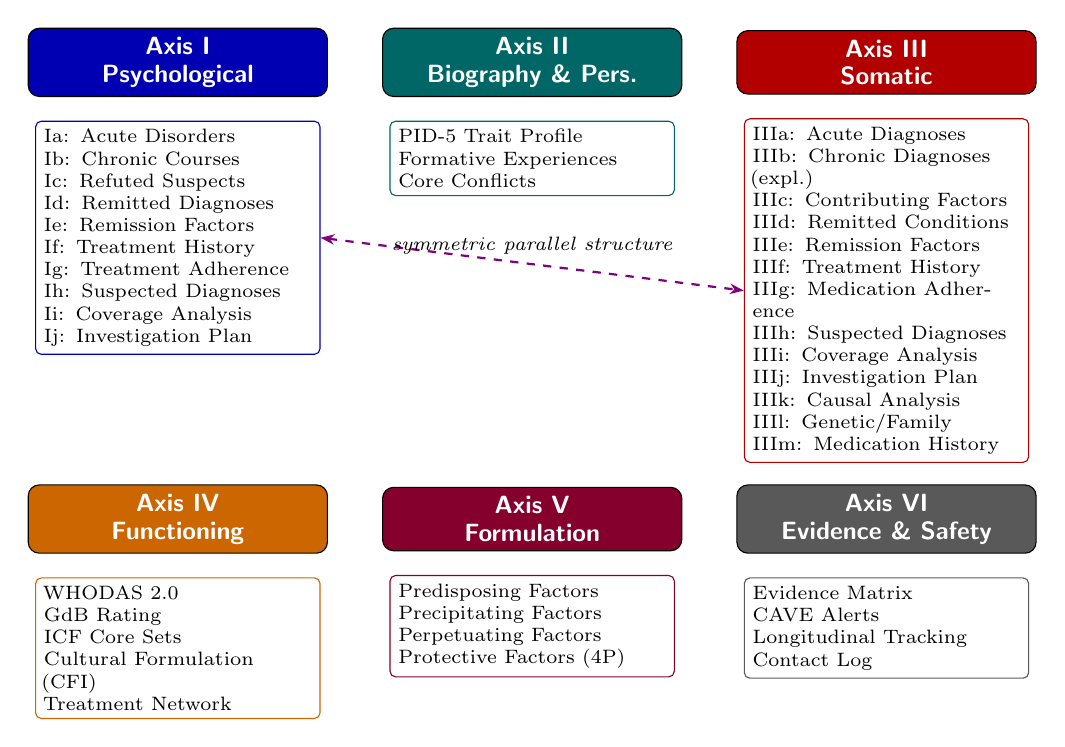
\begin{tikzpicture}[
    axisbox/.style={draw, rounded corners=4pt, minimum width=3.8cm, minimum height=0.7cm,
        font=\sffamily\small\bfseries, text=white, align=center},
    subbox/.style={draw, rounded corners=2pt, minimum width=3.6cm, font=\scriptsize,
        align=left, text width=3.4cm, inner sep=3pt, fill=white},
    >=Stealth
]
% --- Axis I (left) ---
\node[axisbox, fill=blue!70!black] (ax1) at (0,0) {Axis I\\[-1pt]Psychological};
\node[subbox, below=0.3cm of ax1, draw=blue!70!black] (ax1sub) {
    Ia: Acute Disorders\\
    Ib: Chronic Courses\\
    Ic: Refuted Suspects\\
    Id: Remitted Diagnoses\\
    Ie: Remission Factors\\
    If: Treatment History\\
    Ig: Treatment Adherence\\
    Ih: Suspected Diagnoses\\
    Ii: Coverage Analysis\\
    Ij: Investigation Plan
};

% --- Axis II (center-left) ---
\node[axisbox, fill=teal!80!black] (ax2) at (4.5,0) {Axis II\\[-1pt]Biography \& Pers.};
\node[subbox, below=0.3cm of ax2, draw=teal!80!black] (ax2sub) {
    PID-5 Trait Profile\\
    Formative Experiences\\
    Core Conflicts
};

% --- Axis III (right of I, symmetric) ---
\node[axisbox, fill=red!70!black] (ax3) at (9,0) {Axis III\\[-1pt]Somatic};
\node[subbox, below=0.3cm of ax3, draw=red!70!black] (ax3sub) {
    IIIa: Acute Diagnoses\\
    IIIb: Chronic Diagnoses (expl.)\\
    IIIc: Contributing Factors\\
    IIId: Remitted Conditions\\
    IIIe: Remission Factors\\
    IIIf: Treatment History\\
    IIIg: Medication Adherence\\
    IIIh: Suspected Diagnoses\\
    IIIi: Coverage Analysis\\
    IIIj: Investigation Plan\\
    IIIk: Causal Analysis\\
    IIIl: Genetic/Family\\
    IIIm: Medication History
};

% --- Symmetry arrow between I and III ---
\draw[dashed, thick, blue!50!red, {Stealth[length=5pt]}-{Stealth[length=5pt]}]
    (ax1sub.east) -- (ax3sub.west)
    node[midway, above, font=\scriptsize\itshape, text=black] {symmetric parallel structure};

% --- Axis IV (below left) ---
\node[axisbox, fill=orange!80!black] (ax4) at (0,-5.8) {Axis IV\\[-1pt]Functioning};
\node[subbox, below=0.3cm of ax4, draw=orange!80!black] (ax4sub) {
    WHODAS 2.0\\
    GdB Rating\\
    ICF Core Sets\\
    Cultural Formulation (CFI)\\
    Treatment Network
};

% --- Axis V (below center) ---
\node[axisbox, fill=purple!70!black] (ax5) at (4.5,-5.8) {Axis V\\[-1pt]Formulation};
\node[subbox, below=0.3cm of ax5, draw=purple!70!black] (ax5sub) {
    Predisposing Factors\\
    Precipitating Factors\\
    Perpetuating Factors\\
    Protective Factors (4P)
};

% --- Axis VI (below right) ---
\node[axisbox, fill=gray!70!black] (ax6) at (9,-5.8) {Axis VI\\[-1pt]Evidence \& Safety};
\node[subbox, below=0.3cm of ax6, draw=gray!70!black] (ax6sub) {
    Evidence Matrix\\
    CAVE Alerts\\
    Longitudinal Tracking\\
    Contact Log
};

\end{tikzpicture}
\caption{Architecture of the 6-axis model with sub-axes. Axes~I and~III share a symmetric parallel structure (indicated by the dashed arrow).}
\label{fig:architecture}
\end{figure}

\begin{table}[H]
\centering
\caption{Overview of the diagnostic axes of the 6-axis model}
\label{tab:achsen}
\footnotesize
\begin{tabularx}{\textwidth}{@{}L{0.8cm}L{2.1cm}L{3.3cm}Y L{2.2cm}@{}}
\toprule
\textbf{Axis} & \textbf{Designation} & \textbf{Subdivision} & \textbf{Core Content} & \textbf{Typical Profession} \\
\midrule
I & Mental Health Profiles & Ia: Acute Disorders \newline Ib: Chronic Courses \newline Ic: Refuted Suspects \newline Id: Remitted Diagnoses \newline Ie: Remission Factors \newline If: Treatment History \newline Ig: Treatment Adherence \newline Ih: Suspected Diagnoses \newline Ii: Coverage Analysis \newline Ij: Investigation Plan & DSM-5 Cross-Cutting; PHQ-9, PCL-5, ITQ; Differential Diagnosis; Chronification; Temporal Mapping & Psychologist / Psychiatrist \\
\addlinespace
II & Biography \& Personality & Developmental History \newline Formative Experiences \newline Core Conflicts \newline Personality (PID-5) & IQ, Education, Socialization; Life Events; OPD Conflicts; PID-5-BF/+M & Psychologist / Social Worker \\
\addlinespace
III & Medical Synopsis & IIIa: Acute Med. Diagnoses \newline IIIb: Chronic Diagnoses (expl.) \newline IIIc: Contributing Factors \newline IIId: Remitted Conditions \newline IIIe: Remission Factors \newline IIIf: Treatment History \newline IIIg: Medication Adherence \newline IIIh: Suspected Diagnoses \newline IIIi: Coverage Analysis \newline IIIj: Investigation Plan \newline IIIk: Causal Analysis \newline IIIl: Genetic/Family \newline IIIm: Medication History & Biographical Medical History; Causal Analysis Soma--Psyche; Genetic Burden; Pharmacotherapy with Efficacy Rating & Physician / Specialist \\
\addlinespace
IV & Environment \& Functioning & Participation (ICF) \newline Psychosocial Circumstances \newline Contact Network \newline Cultural Formulation & WHODAS~2.0, GdB; Mini-ICF-APP; Stressors; Treatment Network; CFI & Social Worker \\
\addlinespace
V & Condition Model & Predisposing Factors \newline Precipitating Factors \newline Perpetuating Factors \newline Protective Factors \newline Clinical Synthesis & 3P/4P Model; Axis Integration; Treatment Planning; Prognosis & Interdisciplinary Team \\
\addlinespace
VI & Evidence Collection \& Clinical Safety & Evidence Matrix (with assessment) \newline CAVE Alerts \newline Symptom Course \newline Contact Log & Document register with clinical assessment; CAVE alerts; Symptom course; Contact/Observation log & All Professions \\
\bottomrule
\end{tabularx}
\normalsize
\end{table}

\subsection{Axis~I: Mental Health Profiles --- Temporal Diagnostics}
\label{sec:axis1}

Axis~I extends beyond a simple diagnosis list by capturing diagnoses in their temporal dynamics. The division into ten sub-axes (Ia--Ij) enables documentation of the entire diagnostic lifecycle: current acute disorders (Ia), chronic courses with chronification risk (Ib), explicitly refuted diagnostic hypotheses with differential-diagnostic rationale (Ic), remitted diagnoses with documented inactivity (Id), remission factors such as therapy, medication, or spontaneous coping (Ie), complete treatment history including effects and side effects (If), treatment adherence from self-report and collateral perspectives (Ig), active suspected diagnoses as diagnostic hypotheses (Ih), the coverage analysis of unexplained residual symptoms (Ii), and structured investigation plans for next diagnostic steps (Ij).

The ordering of coverage analysis (Ii) before investigation plan (Ij) follows clinical logic: diagnostically unexplained symptoms must first be systematically identified before targeted investigations for their clarification can be planned. The investigation plan thus derives directly from the gaps identified by the coverage analysis.

\textbf{PRO/CONTRA evidence evaluation:} Each diagnosis receives a structured evidence evaluation with explicit documentation of findings supporting (PRO) and opposing (CONTRA) the diagnosis, together with a numerical confidence estimate (0--100\%). This operationalization follows the principle of differential-diagnostic transparency: the clinician must document not only \textit{that} a diagnosis is made, but \textit{why}---and which counterarguments were considered and rejected.

\textbf{Quantitative coverage analysis (Ii):} A symptom--diagnosis matrix quantifies the degree of diagnostic explanation for each symptom through the active diagnoses. The formal definition, thresholds, and sensitivity analysis are presented in detail in Section~\ref{sec:coverage}.

\textbf{Prioritized investigation plan (Ij):} The investigation plan uses a 3-tier prioritization scheme: \textit{Urgent} (to be clarified within 4~weeks---e.g., suicidality assessment, emergency medical diagnostics), \textit{Important} (within 3~months---e.g., neuropsychological testing, differential diagnostics), and \textit{Monitoring} (continuous monitoring---e.g., symptom course under therapy). Each planned investigation is assigned to a specialty and provided with a clinical rationale.

This temporal dimensionality was missing both in Axis~I of the DSM-IV and in the flat listing of the DSM-5.

\subsection{Axis~II: Biography and Dimensional Personality}

Axis~II modernizes personality assessment through dimensional PID-5 trait profiling as recommended by both ICD-11 and the DSM-5 Alternative Model. The ICD-11 model replaces categorical personality disorder types with a severity rating (personality difficulty $\to$ mild $\to$ moderate $\to$ severe), five trait qualifiers (Negative Affectivity, Detachment, Dissociality, Disinhibition, Anankastia), and a Borderline Pattern specifier. The DSM-5 AMPD uses the Level of Personality Functioning Scale (LPFS) for Criterion~A and five trait domains with 25 facets for Criterion~B.

The \textbf{PID-5-BF+M} (36~items, 6~domains, 18~facets) bridges both systems and is available in over 12~languages. Meta-analyses show overall convergence of $r = 0.62$ between the systems, with domain correlations of $r = 0.78$--$0.86$, except for Anankastia ($r = 0.34$), which has no direct AMPD equivalent.

Recent work on integrating the ICD-11 and DSM-5 dimensional systems for personality disorders into a unified taxonomy with non-overlapping traits supports the PID-5-based approach adopted here \citep{Bach2022}.

Beyond dimensional personality assessment (IIa), Axis~II integrates two additional biographical components: \textbf{Formative experiences (IIb)} document life events of biographical significance with life stage and impact on the current situation (e.g., early loss, violence, migration). \textbf{Core conflicts (IIc)} capture recurring intrapsychic themes (e.g., autonomy--dependency conflict, self-worth conflict) as described in the psychodynamic tradition and the OPD system. Both components are implemented as open lists that grow with the diagnostic process, providing essential material for case formulation in Axis~V.

\textbf{Relationship to the DSM-5 AMPD:} The Alternative Model for Personality Disorders is implicitly biaxial (Criterion~A: LPFS functioning level; Criterion~B: pathological traits). The present model adopts Criterion~B (PID-5 traits) in Axis~II but extends it with biographical contextualization (formative experiences, core conflicts), while relocating the functional assessment (LPFS analogue) to Axis~IV (WHODAS~2.0, Mini-ICF-APP). This preserves the AMPD's diagnostic information while distributing it across axes aligned with distinct professional responsibilities.

\subsection{Axis~III: Medical Synopsis --- Symmetric Parallel Structure to Axis~I}
\label{sec:axis3}

A central design principle of the model is the \textbf{structural symmetry} between Axis~I (psychological) and Axis~III (somatic). The rationale is that if Axis~I supports suspected diagnoses, documented refutations, and coverage analyses, Axis~III should offer comparable capabilities for the somatic domain. This symmetry is intended to make multi-professional work more consistent.

Axis~III therefore encompasses 13~sub-axes:

\begin{description}[style=nextline, leftmargin=1.5cm, font=\bfseries]
\item[IIIa--IIIj: Parallel Core Structure] These ten sub-axes follow the basic structure of Axis~I, where sub-axes IIIb (explanatory chronic diagnoses) and IIIc (contributing factors) represent a domain-specific differentiation without a direct equivalent in Axis~I: acute somatic diagnoses (IIIa), chronic somatic diagnoses with fully explanatory character (IIIb), contributing medical factors---somatic findings that promote or exacerbate psychopathology without fully explaining it (IIIc), remitted somatic conditions (IIId), somatic remission factors---surgical interventions, medication, lifestyle changes (IIIe), medical treatment history including surgeries, pharmacotherapy, and side effects (IIIf), medication adherence from medical documentation and patient report (IIIg), medical suspected diagnoses as active diagnostic hypotheses (IIIh), somatic coverage analysis---physical symptoms not explained by any current medical diagnosis (IIIi), and medical investigation plan for further somatic diagnostics (IIIj).
\item[IIIk--IIIm: Axis-III-Specific Sub-Axes] Three sub-axes have no counterpart in Axis~I, as they map the specific soma--psyche relationship: integrated causal analysis---systematic assignment of somatic findings to psychopathology distinguishing full explanation (e.g., hypothyroidism explains depression) from contributing effect (e.g., chronic pain exacerbates anxiety disorder) (IIIk); genetic and family burden---family history for somatic and psychiatric disorders, known genetic predispositions, and where applicable results from exome sequencing (IIIl); medication history and interactions---structured recording of all current and past medications with dosage, unit, purpose/indication, schedule, efficacy rating (0--10), side effects, and potential interactions (IIIm).
\end{description}

\textbf{Note on the IIIb/IIIc design decision:} The explicit differentiation between fully explanatory chronic diagnoses (IIIb) and merely contributing factors (IIIc) integrates causal analysis directly into the classification structure. Refuted medical suspected diagnoses are documented within IIIh (suspected diagnoses) through a status change, analogous to clinical practice where suspected diagnoses are excluded and dismissed with rationale.

\textbf{Note on IIIm:} The medication history as a standalone sub-axis (rather than a mere listing in IIIf) enables structured capture of efficacy profiles, interaction risks, and adherence at the preparation level. This is clinically essential, as polypharmacy and drug interactions are a frequent cause of both somatic and psychiatric complications.

This symmetry ensures that the system functions as a \textit{shared tool} for physicians and psychologists. A physician completing Axis~III has the same diagnostic depth available as a psychologist working in Axis~I.

\subsection{Axis~IV: Environment and Functioning --- ICF Integration and Cultural Formulation}
\label{sec:axis4}

Axis~IV combines multiple validated instruments. The \textbf{WHODAS~2.0} \citep{WHO2010} (WHO Disability Assessment Schedule) captures six domains---Cognition, Mobility, Self-care, Getting Along, Life Activities, and Participation---optionally as 12-item short form (explains 81\% of variance; \citealp{Luciano2010}) or 36-item full version. Psychometric properties are strong: Cronbach's $\alpha = 0.94$--$0.96$, test-retest ICC $= 0.93$--$0.96$.

WHODAS~2.0 and GAF measure \textit{fundamentally different constructs}: GAF conflates symptoms and functioning; WHODAS~2.0 measures disability independently of symptom severity. \citet{Gspandl2018} found \textit{no significant correlation} between self-rated WHODAS~2.0 and GAF in schizophrenia spectrum disorders. The system primarily uses WHODAS~2.0 for disability assessment. The GAF may optionally be retained for backward compatibility but is not a core component.

For the German context, the \textbf{GdB integration} (Grad der Behinderung, degree of disability) is essential. The GdB uses a 20--100 scale ($\geq 50$ = severe disability) and is assessed according to the Versorgungsmedizinische Grunds\"atze (VMG). For international implementations, this sub-axis should be replaced with the equivalent national disability assessment framework (e.g., Disability Adjusted Life Years in WHO contexts, or the Social Security Disability determination in the U.S.).

Three mental-health \textbf{ICF Core Set} families have been developed for depression, bipolar disorder, and schizophrenia \citep{Cieza2004Depression, AyusoMateos2013Bipolar, GomezBenito2018Schizophrenia}: depression (31~brief/121~comprehensive categories), bipolar disorder (19/38), and schizophrenia (25/97). For practical implementation, the \textbf{Mini-ICF-P} rating by \citet{LindenBaron2005} with 13~capacity dimensions is the most efficient tool.

\textbf{Operationalization of ICF integration in Axes~III and~VI:} The ICF coding in the 6-axis model follows a three-stage logic. \textit{First}, on Axis~III (Medical Synopsis), the body functions (ICF Chapter~b) and body structures (ICF Chapter~s) relevant to the somatic-psychological causal analysis (IIIk) are documented---e.g., \texttt{b130} (energy and drive functions), \texttt{b152} (emotional functions), or \texttt{b144} (memory functions). \textit{Second}, Axis~IV captures activities and participation (ICF Chapter~d) and environmental factors (ICF Chapter~e)---operationalized through WHODAS~2.0 (domains d1--d6) and Mini-ICF-APP (13 capacity dimensions, e.g., regularity, flexibility, social competence). \textit{Third}, the evidence matrix (Axis~VI) documents the ICF qualifiers (extent of impairment: 0--4) for each coded functional restriction, enabling quantification over time.

\textbf{Added value beyond WHODAS~2.0 alone:} While WHODAS~2.0 as a global disability instrument captures six domains on a summary scale, the 6-axis model enables \textit{axis-specific differentiation}: functional restrictions are not only quantified but causally attributed to Axes~I (psychological) and~III (somatic). The coverage analysis (Ii/IIIi) additionally identifies functional deficits not explained by any current diagnosis---a dimension that WHODAS~2.0 does not address. The Mini-ICF-APP complements WHODAS~2.0 with disorder-specific capacity profiles directly usable for treatment planning and prognosis in Axis~V (Condition Model).

\subsubsection{Contact Persons and Treatment Network}

Axis~IV also captures the patient's \textbf{contact persons and treatment network}. For each contact person, name, role (parent, partner, GP, specialist, therapist, social worker, guardian, etc.), institution, contact details, and notes are documented. This structured network recording serves multiple purposes: it makes the social support system visible, which is essential for case formulation (Axis~V, protective factors) and treatment planning; it documents the professional network involved for coordination; and it identifies potential sources for collateral histories.

\subsubsection{Cultural Formulation Interview (CFI)}

The DSM-5-TR contains a structured \textbf{Cultural Formulation Interview} (CFI) with 16~core questions across four domains: cultural definition of the problem, cultural perception of cause/context/support, cultural factors in coping, and cultural factors in the clinician--patient relationship. For a model claiming comprehensive biopsychosocial assessment, integration of the CFI as an optional module in Axis~IV is essential. The 12~supplementary CFI modules (for specific populations and contexts) can be activated as needed.

\subsection{Axis~V: Integrated Condition Model --- Operationalized Case Formulation}
\label{sec:axis5}

Axis~V represents a proposed extension not contained in previous systems. The predisposing--precipitating--perpetuating factor model (clinical 3P/4P model) bridges diagnostic classification with case formulation---something no DSM edition has ever contained. \citet{Owen2023} argues that this formulation approach ``disciplines the selection of facts and makes treatment goal-directed.'' The synthesis of all axes---how biology (III), biography (II), and current stressors (IV) interact with psychopathology (I)---is made explicit here.

The model operationalizes case formulation through four structured components:

\begin{description}[style=nextline, leftmargin=1.5cm, font=\bfseries]
\item[Predisposing Factors (P1)] Vulnerability factors that existed before the disorder. Sources: Axis~II (biographical risk factors, personality traits), Axis~III (genetic burden, IIIm), Axis~IV (early psychosocial stress). Coding: factor, source axis, evidence strength (established/probable/possible), evidence (Axis~VI reference).
\item[Precipitating Factors (P2)] Events or changes that triggered disorder onset. Sources: Axis~IV (current stressors, life events), Axis~III (somatic triggers). Coding: factor, temporal relationship, source axis, evidence.
\item[Perpetuating Factors (P3)] Conditions that maintain the disorder. Sources: Axis~I (comorbidities, treatment adherence), Axis~III (untreated somatic findings), Axis~IV (persistent psychosocial stress). Coding: factor, mechanism, modifiability (modifiable/stable), intervention priority.
\item[Protective Factors (P4)] Resources that promote resilience. Sources: Axis~II (personality strengths), Axis~IV (social support, economic resources), Axis~I (remission factors, Ie). Coding: factor, source axis, activatability.
\end{description}

\textbf{Transtheoretical compatibility:} The 3P/4P model is deliberately transtheoretical in design. Behavioral case conceptualizations (e.g., the SORKC model) can be directly translated into the Axis~V structure: stimulus situations correspond to precipitating factors (P2), organism variables to predisposing factors (P1), response patterns and consequences to perpetuating factors (P3). Psychodynamic formulations (OPD conflicts, structural limitations) likewise find their place in P1 and P3. This compatibility is no coincidence but reflects the empirical convergence of different therapeutic schools on common etiological factors.

The link to coverage analysis (Axis~Ii) is central: symptoms not covered by any Axis~I diagnosis are expected to be examined through the Axis~V formulation. Symptoms that are neither diagnostically nor formulationally explained represent remaining diagnostic gaps and trigger the investigation plan (Axis~Ij).

\subsection{Axis~VI: Evidence Collection, CAVE Alerts, and Symptom Course}

Axis~VI has been substantially expanded from the original design and now comprises four components:

\begin{description}[style=nextline, leftmargin=1.5cm, font=\bfseries]
\item[Evidence Matrix] A central document register linking every coded piece of information to evidence (document analysis, interview, testing). Each entry includes, beyond axis reference, document type, and description, an explicit \textbf{assessment field} for the clinical evaluation: an incoming lab report is documented with date, designation, source, \textit{and} clinical interpretation---making transparent how the clinician interprets the finding in the diagnostic context.
\item[CAVE Alerts] A structured warning system for critical clinical risks with cross-axis relevance. Each alert is categorized as: \textit{Drug interaction} (e.g., Lithium + NSAIDs), \textit{Lab artifact} (e.g., CRP elevation due to chronic inflammation, not acute infection), \textit{Contraindication} (e.g., pregnancy with certain medications), \textit{Temporal misattribution} (e.g., symptom onset before or after suspected trigger), \textit{Diagnostic limitation} (e.g., unusable test result), and \textit{Other warning}. Each alert references the affected source axis (I--VI) for immediate contextualization. CAVE alerts are prominently highlighted in red in the overall synopsis.
\item[Longitudinal Symptom Course] Structured documentation of the temporal symptom course: for each relevant symptom, onset (first manifestation), current status (active/remitted/fluctuating), and therapy response (response/non-response/partial response) are recorded.
\item[Contact and Observation Log] A structured protocol for all clinically relevant contacts and observations. Each entry comprises date, contact type (phone call, interview, observation, home visit, collateral history, email/letter), contact person, content, and optional axis reference. The log documents the \textit{process} of information gathering.
\end{description}

\subsection{Multi-Professional Team Assignment}
\label{sec:multiprofessional}

The 6-axis model provides a \textbf{recommended}, non-mandatory assignment of axes to professional groups. Table~\ref{tab:professions} shows an exemplary configuration for interdisciplinary teams. In clinical practice, responsibilities can be flexibly adapted: a psychiatrist with both psychodiagnostic and somatic competence can naturally complete both Axis~I \textit{and} Axis~III; a psychosomatic medicine specialist can serve all six axes. The system \textit{enables} interdisciplinary division of labor but does not \textit{enforce} it.

The value of the assignment lies not in rigid access restrictions but in the \textbf{structured prompt}: the system makes transparent \textit{which} competence is typically needed for which axis. In solo practices or smaller settings, a single professional can work on all axes; in clinics and interdisciplinary teams, the model enables efficient division of labor where each profession works in its domain with identical structural tools. The identical sub-axis structure of Axes~I and~III is not coincidental but a design decision: a physician formulating a somatic suspected diagnosis in IIIh uses exactly the same logic as a psychologist entering a psychological suspected diagnosis in Ih.

\begin{table}[H]
\centering
\caption{Exemplary multi-professional axis assignment (non-mandatory)}
\label{tab:professions}
\begin{tabularx}{\textwidth}{lXX}
\toprule
\textbf{Axis} & \textbf{Typical Profession} & \textbf{Professional Rationale} \\
\midrule
I & Psychologist / Psychiatrist & Psychodiagnostic competence; testing authority \\
\addlinespace
II & Psychologist / Social worker & Biographical history; personality assessment \\
\addlinespace
III & Physician / Specialist & Somatic diagnosis; causal analysis \\
\addlinespace
IV & Social worker & Life-world expertise; ICF competence; participation assessment \\
\addlinespace
V & Interdisciplinary team & Synthesis benefits from all perspectives \\
\addlinespace
VI & All professions & Each participating profession documents its own findings \\
\bottomrule
\end{tabularx}
\end{table}

\subsection{Comorbidity Rules and Diagnostic Hierarchy}
\label{sec:comorbidity}

The system implements three levels of comorbidity rules essential for correct diagnostic decision-making:

\begin{description}[style=nextline, leftmargin=1.5cm, font=\bfseries]
\item[Hierarchical Exclusion Rules] Certain diagnoses exclude others. Example: a schizophrenia diagnosis excludes a concurrent schizoaffective disorder. The system codes these as hard constraints that are automatically checked upon diagnosis entry.
\item[``Due to Another Condition'' Rules] Many DSM-5-TR diagnoses require ruling out that the symptomatology is better explained by another mental disorder, a substance, or a medical condition. These rules are directly implemented through Gatekeeper Steps~1--3 (Section~\ref{sec:gatekeeper}).
\item[Permitted Comorbidities with Prioritization] With 4+ active diagnoses, the system prioritizes by: (1)~clinical urgency (suicidality, psychosis), (2)~severity (Axis~I acute status), (3)~treatability (modifiable perpetuating factors from Axis~V), (4)~chronological order.
\end{description}

\clearpage
\subsection{Complete Sub-Axis Inventory}

Tables~\ref{tab:subaxes_part1}, \ref{tab:subaxes_part2}, and \ref{tab:subaxes_part3} provide a complete inventory of all sub-axes across the six main axes, including associated instruments and data sources.

\begin{table}[H]
\centering
\caption{Sub-axis inventory: Axes I--II}
\label{tab:subaxes_part1}
\begin{CompactLongTable}
\begin{tabular}{@{}L{1.8cm}L{2.4cm}L{5.0cm}L{4.0cm}@{}}
\toprule
\textbf{Axis} & \textbf{Sub-Axis} & \textbf{Description} & \textbf{Instrument / Source} \\
\midrule
I\\Psychological & Ia: Acute Disorders & Current DSM-5-TR/ICD-11 diagnoses with PRO/CONTRA evidence and confidence & DSM-5-TR, ICD-11 \\
 & Ib: Chronic Courses & Long-term diagnoses with chronification risk & Clinical records \\
 & Ic: Refuted Suspects & Explicitly ruled-out diagnoses with differential-diagnostic rationale & Differential diagnosis \\
 & Id: Remitted Diagnoses & Former diagnoses with documented inactivity & Clinical records \\
 & Ie: Remission Factors & Therapy, medication, or spontaneous coping as remission cause & Clinical records \\
 & If: Treatment History & Prior treatments, medications, effects and side effects & Clinical records \\
 & Ig: Treatment Adherence & Adherence from self-report and collateral perspectives & Clinical interview \\
 & Ih: Suspected Diagnoses & Active diagnostic hypotheses (not yet confirmed) & Clinical judgment \\
 & Ii: Coverage Analysis & Symptom--diagnosis coverage percentage (DCI) & Algorithmic (see Section~\ref{sec:coverage}) \\
 & Ij: Investigation Plan & Prioritized next steps (urgent / important / monitoring) & Clinical judgment \\
\midrule
II\\Personality & IIa: PID-5 Dimensional Profile & 5 trait domains, 25 facets & PID-5, PID5BF+ \\
 & IIb: Formative Life Experiences & Biographical events shaping personality development & Clinical interview \\
 & IIc: Core Conflicts & Central relational patterns and conflict themes & OPD-3, clinical formulation \\
\bottomrule
\end{tabular}
\end{CompactLongTable}
\end{table}

\begin{table}[H]
\centering
\caption{Sub-axis inventory: Axis III}
\label{tab:subaxes_part2}
\begin{CompactLongTable}
\begin{tabular}{@{}L{1.8cm}L{2.4cm}L{5.0cm}L{4.0cm}@{}}
\toprule
\textbf{Axis} & \textbf{Sub-Axis} & \textbf{Description} & \textbf{Instrument / Source} \\
\midrule
III\\Somatic & IIIa: Acute Somatic Diagnoses & Current somatic diagnoses with PRO/CONTRA evidence & ICD-11 somatic codes \\
 & IIIb: Chronic Diagnoses (explanatory) & Conditions that fully account for specific symptoms & Clinical records \\
 & IIIc: Contributing Medical Factors & Somatic findings that promote or exacerbate psychopathology & Clinical records \\
 & IIId: Remitted Conditions & Prior somatic conditions with documented inactivity & Clinical records \\
 & IIIe: Remission Factors & Surgical interventions, medication, lifestyle changes as remission causes & Clinical records \\
 & IIIf: Treatment History & Prior medical treatments, surgeries, side effects & Clinical records \\
 & IIIg: Medication Adherence & Adherence from medical documentation and patient report & Clinical records \\
 & IIIh: Suspected Diagnoses & Active medical diagnostic hypotheses & Clinical judgment \\
 & IIIi: Coverage Analysis (Somatic) & Somatic symptom--diagnosis coverage percentage & Algorithmic (see Section~\ref{sec:coverage}) \\
 & IIIj: Somatic Investigation Plan & Medical workup priorities & Clinical judgment \\
 & IIIk: Integrated Causal Analysis & Cross-axis causal pathways (somatic $\leftrightarrow$ psychological) & Interdisciplinary synthesis \\
 & IIIl: Genetic/Family Burden & Hereditary risk factors and family medical history & Family history interview \\
 & IIIm: Medication History & Current and past medications with efficacy ratings & Medication records \\
\bottomrule
\end{tabular}
\end{CompactLongTable}
\end{table}

\begin{table}[H]
\centering
\caption{Sub-axis inventory: Axes IV--VI}
\label{tab:subaxes_part3}
\begin{CompactLongTable}
\begin{tabular}{@{}L{1.8cm}L{2.4cm}L{5.0cm}L{4.0cm}@{}}
\toprule
\textbf{Axis} & \textbf{Sub-Axis} & \textbf{Description} & \textbf{Instrument / Source} \\
\midrule
IV\\Functional\\Status & IVa: WHODAS 2.0 & 6 functional domains (36-item or 12-item version) & WHODAS 2.0 \\
 & IVb: GdB & German disability degree (\textit{Grad der Behinderung}) & VersMedV guidelines \\
 & IVc: ICF Core Sets & Disorder-specific ICF component profiles & ICF Core Sets \\
 & IVd: Cultural Formulation Interview & Cultural context of illness experience & CFI (DSM-5-TR) \\
 & IVe: Treatment Network Register & Contact persons, providers, social support & Structured register \\
\midrule
V\\Case\\Formulation & Va: Predisposing Factors & Vulnerability factors preceding disorder onset & 3P/4P schema \\
 & Vb: Precipitating Factors & Triggering events and stressors & 3P/4P schema \\
 & Vc: Perpetuating Factors & Maintaining mechanisms and feedback loops & 3P/4P schema \\
 & Vd: Protective Factors & Resilience resources and strengths & 3P/4P schema \\
 & Ve: Coverage Gap Integration & Unexplained symptoms from Axes I + III coverage analysis & Cross-axis synthesis \\
\midrule
VI\\Evidence\\\& Safety & VIa: Central Evidence Matrix & Structured evidence fields per diagnosis & System-generated \\
 & VIb: CAVE Clinical Alerts & Cross-axis risk warnings (interactions, contraindications) & Rule-based alerts \\
 & VIc: Longitudinal Symptom Tracking & Repeated measures with therapy response documentation & PHQ-9, GAD-7, PCL-5, etc. \\
 & VId: Contact and Observation Log & Session documentation and process notes & Clinician entries \\
\bottomrule
\end{tabular}
\end{CompactLongTable}
\end{table}

\section{The 6-Step Gatekeeper Logic}
\label{sec:gatekeeper}

The system implements a dynamic queue in which screening findings trigger specific DSM-5-TR/ICD-11 modules. The 6-step sequence maps exactly to the framework published by Michael~B. First in the \textit{DSM-5-TR Handbook of Differential Diagnosis} (2024) (Table~\ref{tab:gatekeeper}).

\begin{table}[H]
\centering
\caption{Alignment of the 6-step gatekeeper logic with First's gold standard}
\label{tab:gatekeeper}
\begin{tabularx}{\textwidth}{clXc}
\toprule
\textbf{Step} & \textbf{System Step} & \textbf{First's Framework} & \textbf{Match} \\
\midrule
1 & Malingering exclusion & Rule out malingering and factitious disorder & Exact \\
\addlinespace
2 & Substance exclusion & Rule out substance etiology & Exact \\
\addlinespace
3 & Medical exclusion & Rule out etiological medical conditions & Exact \\
\addlinespace
4 & Primary category & Determine specific primary disorder(s) & Exact \\
\addlinespace
5 & Adjustment disorder & Differentiate adjustment disorders & Exact \\
\addlinespace
6 & Functional threshold & Boundary with ``no mental disorder'' & Conceptual \\
\bottomrule
\end{tabularx}
\end{table}

\citet{First2024} describes this framework as the definitive macro-level diagnostic process. His Handbook further contains \textbf{30 symptom-oriented decision trees} (two added in the TR edition for dissociative symptoms and repetitive pathological behaviors) and \textbf{67 differential diagnosis tables}, all following this sequence.

\textbf{Note on Step~6 (``conceptual''):} While Steps~1--5 can be mapped algorithmically, Step~6---drawing the boundary between a normal stress response and a mental disorder---is inherently a clinical judgment decision. The system supports this through structured functional data (WHODAS~2.0, Mini-ICF-APP from Axis~IV) and the Cross-Cutting thresholds, but cannot fully automate the clinical decision. This epistemic boundary is explicitly communicated.

\begin{figure}[ht]
\centering
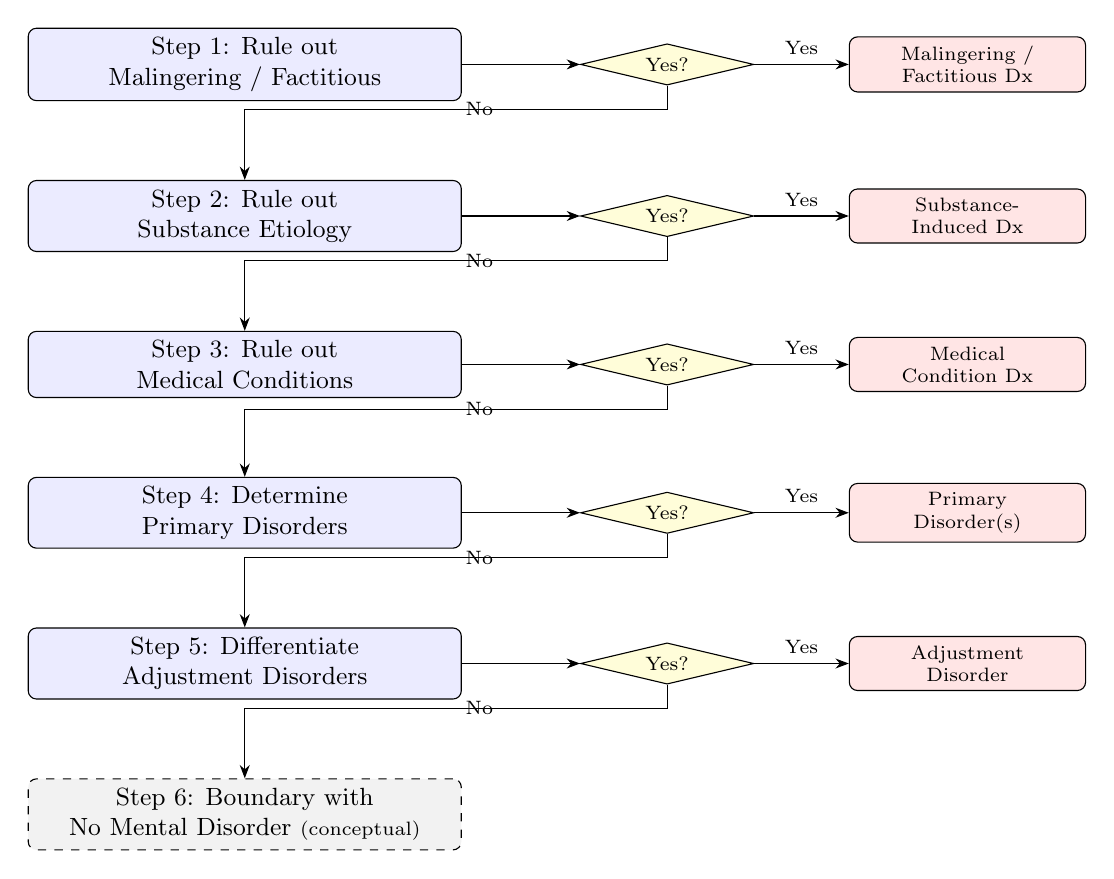
\begin{tikzpicture}[
    stepbox/.style={draw, rounded corners=3pt, minimum width=5.5cm, minimum height=0.8cm,
        font=\small, align=center, fill=blue!8},
    decision/.style={diamond, draw, aspect=2.2, minimum width=2.2cm,
        font=\scriptsize, align=center, fill=yellow!15, inner sep=1pt},
    exitbox/.style={draw, rounded corners=3pt, minimum width=3cm, minimum height=0.6cm,
        font=\scriptsize, align=center, fill=red!10},
    conceptual/.style={draw, rounded corners=3pt, dashed, minimum width=5.5cm, minimum height=0.8cm,
        font=\small, align=center, fill=gray!10},
    >=Stealth, node distance=1.2cm
]

% Steps
\node[stepbox] (s1) {Step 1: Rule out\\Malingering / Factitious};
\node[decision, right=1.5cm of s1] (d1) {Yes?};
\node[exitbox, right=1.2cm of d1] (e1) {Malingering /\\Factitious Dx};

\node[stepbox, below=1.0cm of s1] (s2) {Step 2: Rule out\\Substance Etiology};
\node[decision, right=1.5cm of s2] (d2) {Yes?};
\node[exitbox, right=1.2cm of d2] (e2) {Substance-\\Induced Dx};

\node[stepbox, below=1.0cm of s2] (s3) {Step 3: Rule out\\Medical Conditions};
\node[decision, right=1.5cm of s3] (d3) {Yes?};
\node[exitbox, right=1.2cm of d3] (e3) {Medical\\Condition Dx};

\node[stepbox, below=1.0cm of s3] (s4) {Step 4: Determine\\Primary Disorders};
\node[decision, right=1.5cm of s4] (d4) {Yes?};
\node[exitbox, right=1.2cm of d4] (e4) {Primary\\Disorder(s)};

\node[stepbox, below=1.0cm of s4] (s5) {Step 5: Differentiate\\Adjustment Disorders};
\node[decision, right=1.5cm of s5] (d5) {Yes?};
\node[exitbox, right=1.2cm of d5] (e5) {Adjustment\\Disorder};

\node[conceptual, below=1.0cm of s5] (s6) {Step 6: Boundary with\\No Mental Disorder \textnormal{\scriptsize(conceptual)}};

% Arrows: step to decision
\draw[->] (s1) -- (d1);
\draw[->] (s2) -- (d2);
\draw[->] (s3) -- (d3);
\draw[->] (s4) -- (d4);
\draw[->] (s5) -- (d5);

% Arrows: decision to exit (Yes)
\draw[->] (d1) -- node[above, font=\scriptsize] {Yes} (e1);
\draw[->] (d2) -- node[above, font=\scriptsize] {Yes} (e2);
\draw[->] (d3) -- node[above, font=\scriptsize] {Yes} (e3);
\draw[->] (d4) -- node[above, font=\scriptsize] {Yes} (e4);
\draw[->] (d5) -- node[above, font=\scriptsize] {Yes} (e5);

% Arrows: decision No -> next step
\draw[->] (d1.south) -- ++(0,-0.3) -| node[near start, right, font=\scriptsize] {No} (s2.north);
\draw[->] (d2.south) -- ++(0,-0.3) -| node[near start, right, font=\scriptsize] {No} (s3.north);
\draw[->] (d3.south) -- ++(0,-0.3) -| node[near start, right, font=\scriptsize] {No} (s4.north);
\draw[->] (d4.south) -- ++(0,-0.3) -| node[near start, right, font=\scriptsize] {No} (s5.north);
\draw[->] (d5.south) -- ++(0,-0.3) -| node[near start, right, font=\scriptsize] {No} (s6.north);

\end{tikzpicture}
\caption{6-step gatekeeper logic for differential diagnosis, based on \citet{First2024}. Step~6 is marked as conceptual because the boundary between normal variation and mental disorder requires clinical judgment.}
\label{fig:gatekeeper}
\end{figure}

\section{Cross-Cutting Screening}
\label{sec:screening}

The DSM-5 Cross-Cutting Symptom Measures form the backbone of the screening architecture. The \textbf{Level-1 adult measure} contains \textbf{23~items across 13~domains}: Depression (2), Anger (1), Mania (2), Anxiety (3), Somatic Symptoms (2), Suicidality (1), Psychosis (2), Sleep Problems (1), Memory (1), Repetitive Thoughts and Behaviors (2), Dissociation (1), Personality Functioning (2), and Substance Use (3). Each item uses a 5-point Likert scale (0~= none to 4~= severe).

The threshold logic is clinically calibrated: \textbf{Most domains trigger Level~2 at $\geq 2$ (mild)}, but three safety-critical domains---Suicidality, Psychosis, and Substance Use---\textbf{trigger at $\geq 1$ (slight)}. This asymmetry reflects the clinical imperative to never overlook even minimal endorsement of dangerous symptoms.

Level-2 measures refer to specific validated instruments: PROMIS Depression Short Form, PROMIS Anxiety Short Form, Altman Self-Rating Mania Scale (ASRM), PHQ-15 for somatic symptoms, PROMIS Sleep Disturbance, adapted FOCI Severity Scale for OCD, and adapted NIDA-Modified ASSIST for substance use. Five domains (Suicidality, Psychosis, Memory, Dissociation, Personality Functioning) have \textit{no official Level-2 measures}---the APA recommends clinical evaluation for these.

The DSM-5 Field Trials \citep{Narrow2013} demonstrated \textbf{good to excellent test-retest reliability} (ICC~0.64--0.97) for most items.

\subsection{Child and Adolescent Version}
\label{sec:screening_ca}

The DSM-5 Cross-Cutting system includes a separate \textbf{parent-report version for children and adolescents} (ages 6--17) with \textbf{25~items across 12~domains}. The ``Personality Functioning'' domain is omitted for developmental reasons; instead, irritability and anger are weighted more heavily. A complete implementation requires the pediatric variant as a separate entry pathway and age-appropriate Level-2 instruments.

The present system prefers \textbf{exclusively freely available instruments}; the proprietary CBCL/YSR complex \citep{Achenbach2001} is acknowledged as a reference standard but replaced by license-free alternatives. Table~\ref{tab:instrumente_ca} lists the recommended set of free child/adolescent (C/A) instruments in parallel to the adult matrix (Table~\ref{tab:instruments}).

\begin{table}[htbp]
\centering
\caption{Free screening instruments for children and adolescents (C/A matrix)}
\label{tab:instrumente_ca}
\begin{CompactLongTable}
\begin{tabular}{@{}L{2.4cm}L{2.4cm}L{0.9cm}L{1.5cm}L{2.0cm}L{1.5cm}@{}}
\toprule
\textbf{Domain} & \textbf{Instrument} & \textbf{Items} & \textbf{Age range} & \textbf{Cutoff / Norm} & \textbf{Cost} \\
\midrule
Cross-Cutting (Parent) & DSM-5 XC L1 Parent & 25 & 6--17 & $\geq 1$/$\geq 2$ triage & Free \\
\addlinespace
Gen. psychosoc. screen & SDQ (Self/Parent) & 25 & 4--17 & $\geq 20$ (Total) & Free \\
\addlinespace
Depression & PHQ-9 mod.\ (PHQ-A) & 9 & 11--17 & $\geq 11$ & Free \\
\addlinespace
Anxiety + Depression & RCADS-25 & 25 & 8--18 & $T \geq 65$ & Free \\
\addlinespace
Anxiety (multidim.) & SCARED-C & 41 & 8--18 & $\geq 25$ & Free \\
\addlinespace
PTSD & CPSS-V / CRIES-8 & 20 / 8 & 7--18 & $\geq 31$ / $\geq 17$ & Free \\
\addlinespace
Substance use & CRAFFT 2.1+N & 6+3 & 12--21 & $\geq 2$ & Free \\
\addlinespace
ADHD & SNAP-IV-26 & 26 & 6--18 & Subscale mean & Free \\
\addlinespace
Autism & AQ-10 Adolescent/Child & 10 & 4--15 & $\geq 6$ & Free \\
\addlinespace
OCD & CY-BOCS-SR & 10 & 8--18 & $\geq 16$ & Free \\
\addlinespace
Suicidality & C-SSRS Pediatric & 6 & $\geq 5$ & Any endorse.\ & Free \\
\addlinespace
Eating disorders & SCOFF (from $\sim$age 13) & 5 & 13--18 & $\geq 2$ & Free \\
\bottomrule
\end{tabular}
\end{CompactLongTable}
\end{table}

This selection preserves the diagnostic logic of the adult matrix (domain-oriented, cutoff-based) while substituting each instrument with a developmentally validated, license-free C/A variant. For safety-critical domains (suicidality, substance use, psychosis), the same lower triage threshold applies. The split between \textbf{self-report} (from $\sim$ages 8--11) and \textbf{parent report} (ages 6--17; obligatory for younger children) follows the established convention of pediatric psychometrics.

\subsection{Comprehensive Screening Instrument Matrix}

Table~\ref{tab:instruments} shows the recommended instruments for all major diagnostic domains.

\begin{table}[htbp]
\centering
\caption{Screening instrument matrix}
\label{tab:instruments}
\begin{CompactLongTable}
\begin{tabular}{@{}L{2.4cm}L{2.0cm}L{0.9cm}L{1.6cm}L{2.5cm}L{1.1cm}@{}}
\toprule
\textbf{Domain} & \textbf{Instrument} & \textbf{Items} & \textbf{Cutoff} & \textbf{Sens./Spec.} & \textbf{Cost} \\
\midrule
Depression & PHQ-9 & 9 & $\geq 10$ & 88\%/88\% & Free \\
\addlinespace
Anxiety & GAD-7 & 7 & $\geq 10$ & 89\%/82\% & Free \\
\addlinespace
PTSD (DSM-5) & PCL-5 & 20 & 31--33 & 85--95\%/82--90\% & Free \\
\addlinespace
PTSD/CPTSD (ICD-11) & ITQ & 18 & Algorithm & Excellent & Free \\
\addlinespace
Psychosis risk & PQ-16 & 16 & $\geq 6$ & 87\%/87\% & Free \\
\addlinespace
Bipolar screening & MDQ & 15 & $\geq 7$ & 73\%/90\% & Free \\
\addlinespace
ADHD & ASRS~v1.1 & 6 & $\geq 4$ & 69\%/99.5\% & Free \\
\addlinespace
Autism & AQ-10 & 10 & $\geq 6$ & 88\%/91\% & Free \\
\addlinespace
Alcohol use & AUDIT & 10 & $\geq 8$ & 92\%/94\% & Free \\
\addlinespace
Drug use & DAST-10 & 10 & $\geq 3$ & 98\%/91\% & Free \\
\addlinespace
Personality & PID-5-BF & 25 & Dimensional & N/A & Free \\
\addlinespace
Suicidality & C-SSRS & 6 & Any endors. & Risk classif. & Free \\
\addlinespace
OCD & OCI-R & 18 & $\geq 21$ & Good & Free \\
\addlinespace
Somatization & SSS-8 & 8 & $\geq 12$ & Comparable & Free \\
\addlinespace
Dissociation & DES-II & 28 & $\geq 30$ & 74\%/80\% & Free \\
\addlinespace
Eating disorders & SCOFF & 5 & $\geq 2$ & 84\%/90\% & Free \\
\addlinespace
Eating dis. (detailed) & EDE-QS & 12 & $\geq 15$ & Good/Good & Free \\
\addlinespace
Sleep disorders & ISI & 7 & $\geq 15$ & 82\%/82\% & Free \\
\addlinespace
Functioning & WHODAS 2.0 (12) & 12 & Dimensional & N/A & Free \\
\bottomrule
\end{tabular}
\end{CompactLongTable}
\end{table}

All recommended instruments are \textbf{freely available}---no licensing costs impede implementation. The selection is based on the respective validation publications: PHQ-9 \citep{Levis2019}, GAD-7 \citep{Spitzer2006}, PCL-5 \citep{Blevins2015}, ITQ \citep{Cloitre2018}, PQ-16 \citep{Ising2012}, ASRS \citep{Kessler2005}, AQ-10 \citep{Allison2012}, AUDIT \citep{Saunders1993}, PID-5 \citep{OltmannsWidiger2018, Riegel2021}, C-SSRS \citep{Posner2011}, OCI-R \citep{Foa2002}, SSS-8 \citep{Gierk2014}, DES-II \citep{CarlsonPutnam1993}, SCOFF \citep{Morgan1999}, ISI \citep{Morin2011}. For inter-rater reliability of categorical DSM-5 diagnoses, see \citet{Regier2013} and \citet{Aboraya2006}.

\section{Critical Divergences Between DSM-5-TR and ICD-11}
\label{sec:divergences}

The system must encode five critical divergences between the classification systems \citep{Keeley2016}.

\subsection{Schizophrenia Duration}

DSM-5-TR (295.90/F20.x) requires \textbf{6~months} of continuous signs including at least 1~month of active symptoms, while ICD-11 (6A20) requires only \textbf{1~month}. A patient may thus meet ICD-11 criteria for schizophrenia but only receive a schizophreniform disorder diagnosis under DSM-5.

\subsection{PTSD Architecture}

DSM-5-TR uses \textbf{4~clusters with 20~symptoms} (Intrusion $\geq$1/5, Avoidance $\geq$1/2, Negative Cognitions $\geq$2/7, Arousal $\geq$2/6). ICD-11 uses a deliberately narrower model: \textbf{3~clusters with 6~core symptoms}. ICD-11 then adds \textbf{Complex PTSD (6B41)} as a distinct diagnosis requiring all PTSD criteria plus three disturbances of self-organization (affect dysregulation, negative self-concept, relationship difficulties).

\subsection{Personality Disorders}

ICD-11 completely replaced categorical types with a dimensional model. The DSM-5 Alternative Model for Personality Disorders (AMPD) uses the LPFS for Criterion~A (functioning level) and five trait domains with 25 facets for Criterion~B (pathological traits). The PID-5-BF+M bridges both systems. \textbf{Relationship to Axis~II of the present model:} The AMPD itself is implicitly biaxial (functioning level + traits). Axis~II of the 6-axis model adopts the trait dimension (PID-5) but extends it with biographical contextualization (formative experiences, core conflicts) and relocates the functioning level (LPFS analogue) to Axis~IV (WHODAS~2.0, Mini-ICF-APP). This fully preserves the AMPD's diagnostic information but distributes it across axes aligned with distinct professional responsibilities.

\subsection{Gaming Disorder}

ICD-11 (6C51) uses a monothetic approach (all 4~criteria required; $\geq 12$~months). DSM-5-TR lists Internet Gaming Disorder only as a ``Condition for Further Study'' with a polythetic approach ($\geq 5$ of 9~criteria). Concordance: $\kappa = 0.80$, but ICD-11 has a higher diagnostic threshold (prevalence 2.7\% vs.\ DSM-5 5.2\%).

\subsection{Prolonged Grief Disorder}

ICD-11 (6B42) and DSM-5-TR (Prolonged Grief Disorder, newly added) both encode prolonged grief disorder, but differ in time criterion (ICD-11: 6~months; DSM-5-TR: 12~months) and symptom configuration. The system must accommodate both variants.

\section{The Coverage Analysis: A Proposed Approach}
\label{sec:coverage}

The coverage analysis (\textit{Coverage Analysis}) represents a central proposed component of the system. We are not aware of directly comparable implementations, although related approaches exist (e.g., Bayesian symptom--diagnosis assignment in OPCRIT). The concept encompasses the systematic identification of symptoms not explained by current diagnoses.

The closest existing parallels are: comorbidity detection algorithms that flag symptoms indicating additional diagnoses; First's differential diagnosis tables \citep{First2024}, which compare overlapping presentations; and transdiagnostic frameworks such as HiTOP, in which symptoms are modeled as network nodes. \citet{PlanaRipoll2019} demonstrated empirically that most mental disorders co-occur far more frequently than expected by chance---\textbf{prior diagnosis of any mental disorder substantially increased the risk of all other mental disorders}---which supports the rationale for a systematic coverage analysis tool.

\subsection{Formal Definition of Coverage Analysis}

Let $S = \{s_1, \ldots, s_n\}$ be the set of observed symptoms and $D = \{d_1, \ldots, d_m\}$ the set of established diagnoses. For each symptom $s_i$, define the coverage function $c(s_i) = \max_{d_j \in D} w(s_i, d_j)$, where $w(s_i, d_j) \in [0, 1]$ represents the weight of symptom $s_i$ in diagnosis $d_j$ as defined by the diagnostic criteria. The total coverage---hereafter termed the \textbf{Diagnostic Coverage Index (DCI)}---is then $C_{\text{total}} = \frac{1}{n} \sum_{i=1}^{n} c(s_i)$. Symptom weights are derived from the diagnostic criteria of DSM-5-TR and ICD-11. Criteria are weighted according to diagnostic salience: cardinal symptoms receive high weights ($w \geq 0.8$), while nonspecific symptoms receive lower weights ($0.3 \leq w \leq 0.7$). This initial weighting scheme is heuristic and requires empirical calibration in future work. Overlapping diagnoses are handled by assigning each symptom to the diagnosis providing maximum coverage. The choice of the max function (rather than, e.g., a weighted mean or Bayesian posterior probability) is deliberately conservative: it asks whether \textit{at least one} diagnosis adequately explains the symptom, thereby avoiding the summation of partial explanations that could yield falsely elevated coverage scores. This approach reflects clinical practice, where a symptom is considered ``explained'' when it can be attributed to an established diagnostic entity. Alternative aggregation functions (weighted sum, Bayesian posterior) should be systematically compared in future studies.

\subsection{Threshold Rationale and Sensitivity}

The proposed thresholds (85\%/60\%) should be understood as \textit{preliminary, heuristic starting values} based on analogies to related but methodologically distinct metrics: (1)~In somatic medicine, diagnostic sensitivities $\geq$85\% are considered clinically acceptable for screening purposes \citep{Levis2019}; this threshold was transferred to diagnostic coverage. (2)~The lower threshold of 60\% is modeled on the convention that Fleiss'~$\kappa$ values $<$0.6 are classified as ``insufficient agreement.'' It must be explicitly noted that diagnostic coverage is a different construct from screening sensitivity or inter-rater agreement; the analogies serve merely as orienting reference points, not as methodological justification. These starting values need empirical calibration in at least three clinical cohorts (inpatient, outpatient, somatically comorbid). Regarding sensitivity of the overall metric: since $C_{\text{total}}$ is an arithmetic mean over $n$ symptoms, a single weight change of $\Delta w$ shifts the total by $\Delta C = \Delta w / n$. For typical symptom counts ($n = 8$--$15$), a misestimation of a single weight by $\pm 0.2$ produces an overall shift of only $\pm 1.3$--$2.5$ percentage points---suggesting limited sensitivity to moderate weighting errors, while also showing that with few symptoms ($n < 5$) the metric becomes unstable.

\subsection{Implementation}

The implementation works as follows: (1)~collection of all confirmed symptoms across all screening instruments, (2)~assignment of each symptom to the diagnostic criteria it fulfills, (3)~calculation of a coverage percentage per symptom quantifying the degree of diagnostic explanation, (4)~classification as fully covered ($\geq$85\%), partially covered (60--84\%), or insufficiently covered ($<$60\%), (5)~calculation of a total coverage score as a weighted mean across all symptoms, (6)~presentation of results as a symptom--diagnosis matrix with visual highlighting of diagnostic gaps. The 4P model (Axis~V) serves as a natural complement: symptoms not covered by Axis~I diagnoses (Axis~Ii) should be explainable through the Axis~V formulation; those that are not represent genuine diagnostic gaps and lead to the prioritized investigation plan (Axis~Ij).

The quantitative metric (e.g., ``total coverage: $\sim$88\%'') provides the clinician with immediate feedback on the completeness of their diagnostic work. Related approaches exist in Bayesian diagnostic systems (e.g., DXplain, Isabel Healthcare), which perform symptom--diagnosis assignments; the specific contribution of the present coverage analysis lies in the transparent, percentage-based presentation as a clinical quality assurance metric.

It should be noted that the term ``coverage analysis'' has been used in medical informatics primarily for terminological mapping between classification systems (e.g., ICF vs.\ SNOMED CT for disability assessment). The present model reconceptualizes coverage analysis as a clinical quality assurance metric: rather than measuring overlap between terminologies, it quantifies the proportion of a patient's symptom profile explained by current diagnoses.

\begin{figure}[ht]
\centering
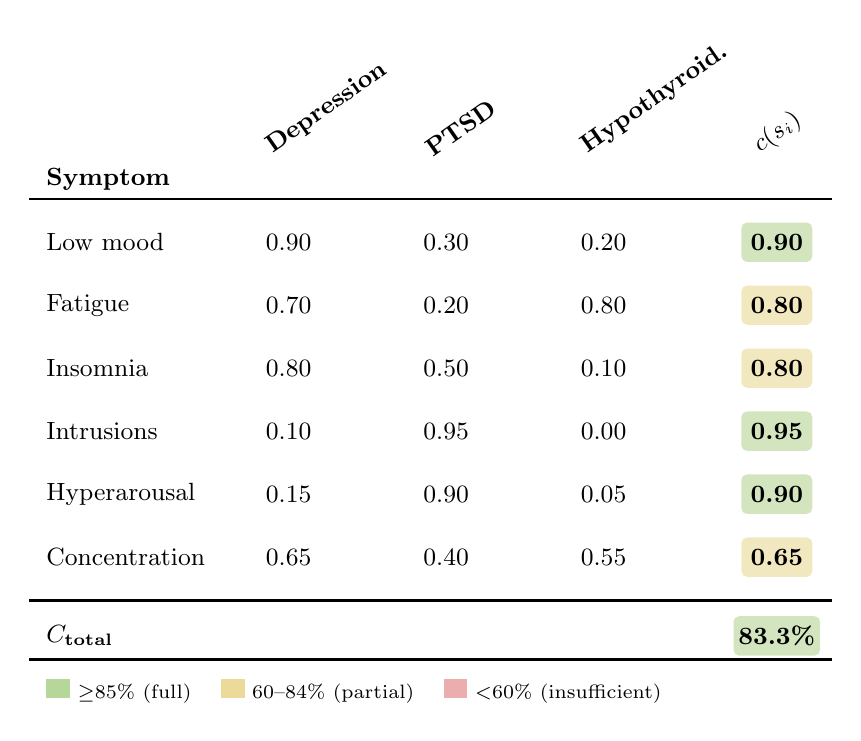
\begin{tikzpicture}[
    font=\small
]
% Define colors
\definecolor{covgreen}{RGB}{76,153,0}
\definecolor{covyellow}{RGB}{204,163,0}
\definecolor{covred}{RGB}{204,51,51}

% Column positions
\def\colA{3.2}   % Depression
\def\colB{5.2}   % PTSD
\def\colC{7.2}   % Hypothyroidism
\def\colD{9.4}   % Coverage c(s_i)

% Row positions (top to bottom)
\def\rowH{6.0}   % Header
\def\rowA{5.2}   % Low mood
\def\rowB{4.4}   % Fatigue
\def\rowC{3.6}   % Insomnia
\def\rowD{2.8}   % Intrusions
\def\rowE{2.0}   % Hyperarousal
\def\rowF{1.2}   % Concentration
\def\rowT{0.2}   % Total

% Header row
\node[font=\small\bfseries, anchor=west] at (0,\rowH) {Symptom};
\node[font=\small\bfseries, rotate=35, anchor=south west] at (\colA-0.2,\rowH+0.1) {Depression};
\node[font=\small\bfseries, rotate=35, anchor=south west] at (\colB-0.2,\rowH+0.1) {PTSD};
\node[font=\small\bfseries, rotate=35, anchor=south west] at (\colC-0.2,\rowH+0.1) {Hypothyroid.};
\node[font=\small\bfseries, rotate=35, anchor=south west] at (\colD-0.2,\rowH+0.1) {$c(s_i)$};

% Horizontal rules
\draw[thick] (-0.1,\rowH-0.25) -- (\colD+0.7,\rowH-0.25);
\draw[thick] (-0.1,\rowT-0.3) -- (\colD+0.7,\rowT-0.3);
\draw[thick] (-0.1,\rowT+0.45) -- (\colD+0.7,\rowT+0.45);

% Helper for colored cell
% Row A: Low mood
\node[anchor=west] at (0,\rowA) {Low mood};
\node at (\colA,\rowA) {0.90};
\node at (\colB,\rowA) {0.30};
\node at (\colC,\rowA) {0.20};
\fill[covgreen, opacity=0.25, rounded corners=2pt] (\colD-0.45,\rowA-0.25) rectangle (\colD+0.45,\rowA+0.25);
\node[font=\small\bfseries] at (\colD,\rowA) {0.90};

% Row B: Fatigue
\node[anchor=west] at (0,\rowB) {Fatigue};
\node at (\colA,\rowB) {0.70};
\node at (\colB,\rowB) {0.20};
\node at (\colC,\rowB) {0.80};
\fill[covyellow, opacity=0.25, rounded corners=2pt] (\colD-0.45,\rowB-0.25) rectangle (\colD+0.45,\rowB+0.25);
\node[font=\small\bfseries] at (\colD,\rowB) {0.80};

% Row C: Insomnia
\node[anchor=west] at (0,\rowC) {Insomnia};
\node at (\colA,\rowC) {0.80};
\node at (\colB,\rowC) {0.50};
\node at (\colC,\rowC) {0.10};
\fill[covyellow, opacity=0.25, rounded corners=2pt] (\colD-0.45,\rowC-0.25) rectangle (\colD+0.45,\rowC+0.25);
\node[font=\small\bfseries] at (\colD,\rowC) {0.80};

% Row D: Intrusions
\node[anchor=west] at (0,\rowD) {Intrusions};
\node at (\colA,\rowD) {0.10};
\node at (\colB,\rowD) {0.95};
\node at (\colC,\rowD) {0.00};
\fill[covgreen, opacity=0.25, rounded corners=2pt] (\colD-0.45,\rowD-0.25) rectangle (\colD+0.45,\rowD+0.25);
\node[font=\small\bfseries] at (\colD,\rowD) {0.95};

% Row E: Hyperarousal
\node[anchor=west] at (0,\rowE) {Hyperarousal};
\node at (\colA,\rowE) {0.15};
\node at (\colB,\rowE) {0.90};
\node at (\colC,\rowE) {0.05};
\fill[covgreen, opacity=0.25, rounded corners=2pt] (\colD-0.45,\rowE-0.25) rectangle (\colD+0.45,\rowE+0.25);
\node[font=\small\bfseries] at (\colD,\rowE) {0.90};

% Row F: Concentration
\node[anchor=west] at (0,\rowF) {Concentration};
\node at (\colA,\rowF) {0.65};
\node at (\colB,\rowF) {0.40};
\node at (\colC,\rowF) {0.55};
\fill[covyellow, opacity=0.25, rounded corners=2pt] (\colD-0.45,\rowF-0.25) rectangle (\colD+0.45,\rowF+0.25);
\node[font=\small\bfseries] at (\colD,\rowF) {0.65};

% Total row
\node[anchor=west, font=\small\bfseries] at (0,\rowT) {$C_{\text{total}}$};
\fill[covgreen, opacity=0.25, rounded corners=2pt] (\colD-0.55,\rowT-0.25) rectangle (\colD+0.55,\rowT+0.25);
\node[font=\small\bfseries] at (\colD,\rowT) {83.3\%};

% Legend
\node[anchor=west, font=\scriptsize] at (0,-0.5) {%
    \tikz\fill[covgreen, opacity=0.4] (0,0) rectangle (0.3,0.25); \(\geq\)85\% (full) \quad
    \tikz\fill[covyellow, opacity=0.4] (0,0) rectangle (0.3,0.25); 60--84\% (partial) \quad
    \tikz\fill[covred, opacity=0.4] (0,0) rectangle (0.3,0.25); $<$60\% (insufficient)
};

\end{tikzpicture}
\caption{Illustrative coverage analysis matrix. Each cell shows the weight $w(s_i, d_j)$; the coverage column shows $c(s_i) = \max_j w(s_i, d_j)$. The total coverage score $C_{\text{total}} = 83.3\%$ indicates partial overall coverage, suggesting further diagnostic investigation is warranted.}
\label{fig:coverage}
\end{figure}

The coverage analysis is symmetrically implemented in Axis~III as well (sub-axis~IIIi): physical symptoms not explained by any current somatic diagnosis are systematically identified and lead to the medical investigation plan (sub-axis~IIIj).


\section{Dimensional Integration: HiTOP and RDoC as Complementary Perspectives}
\label{sec:dimensional}

While the coverage analysis quantifies completeness \textit{within} categorical diagnostics, dimensional frameworks address a complementary limitation: the artificial boundary between diagnostic categories \citep{Rosenman2003}. The 6-axis model is primarily based on categorical diagnostics (DSM-5-TR/ICD-11) but already contains dimensional elements (PID-5, WHODAS~2.0). Two further dimensional frameworks deserve integration as complementary layers:

\subsection{HiTOP (Hierarchical Taxonomy of Psychopathology)}

The Hierarchical Taxonomy of Psychopathology \citep{Kotov2017, Kotov2022, Krueger2018} organizes mental disorders empirically-hierarchically into six spectra: Internalizing (Depression, Anxiety, PTSD), Thought Disorder (Psychosis, Mania), Disinhibited Externalizing (Substance Use, Impulse Control), Antagonistic Externalizing (Antisocial Behavior), Detachment (Social Withdrawal, Anhedonia), and Somatoform (Somatic Symptoms). The system's Cross-Cutting results are mapped directly onto HiTOP spectra and visualized as a radar chart. The mapping uses the maximum expression of the associated Cross-Cutting domains:

\begin{itemize}[noitemsep]
\item Internalizing = max(Depression, Anxiety, Sleep)
\item Thought Disorder = max(Psychosis, Mania, Dissociation)
\item Disinhibited Externalizing = max(Substance)
\item Antagonistic Externalizing = max(Anger)
\item Detachment = max(Personality/Withdrawal)
\item Somatoform = max(Somatic)
\end{itemize}

\textbf{Note on HiTOP mapping:} The assignments follow the current HiTOP consensus \citep{Kotov2021}: mania is assigned to the Thought Disorder spectrum (not Disinhibited Externalizing), as manic episodes in the hierarchical factor structure primarily load on the Thought Disorder factor. Dissociation is also assigned to Thought Disorder, consistent with empirical evidence for a close association with psychotic experiences. The Somatoform spectrum uses exclusively the somatic Cross-Cutting domain; depression-associated somatic burden is captured through the Internalizing spectrum. These mappings should be understood as approximations, as the Cross-Cutting domains were not developed for HiTOP scoring.

This automatic computation requires \textit{no additional data collection}---the domain scores already captured in the Cross-Cutting screening (Section~\ref{sec:screening}) are directly reused. It must be emphasized, however, that this mapping represents a \textit{rough approximation}: the Cross-Cutting domains were not developed for HiTOP mapping, and the max function only incompletely captures the factor-analytically derived spectra. The presentation as a radar chart (visually distinct from the PID-5 personality profile) can promote recognition of transdiagnostic patterns invisible in purely categorical diagnostics, but should be interpreted as exploratory visualization, not as validated measurement.

In summary, the described mapping represents an initial approximation that should be refined with increasing empirical evidence toward HiTOP-conforming assessments \citep{Kotov2021}.

\subsection{RDoC (Research Domain Criteria)}

The Research Domain Criteria of the NIMH \citep{Insel2010} define six domains (Negative Valence, Positive Valence, Cognitive Systems, Social Processes, Arousal/Regulatory, Sensorimotor) with seven levels of analysis (Genes, Molecules, Cells, Circuits, Physiology, Behavior, Self-Report). For a clinical system, RDoC is primarily relevant as \textit{research annotation}: when biomarker data are available (e.g., cortisol profiles, neuroimaging), these can be assigned to RDoC domains. The APA Future DSM Strategic Committee is explicitly exploring biomarker integration---the system is prepared for this.

A separate concept paper describes the detailed architecture of the dimensional integration.

\section{Technical Architecture of the Python Implementation}
\label{sec:technik}

\subsection{Hierarchical State Machines as Decision Engine}

After evaluating four architectural approaches---AnyTree, state machines, rule engines, and behavior trees---\textbf{Hierarchical State Machines (HSMs)} using the Python library \texttt{transitions} emerged as the most practical choice for the present prototype of a psychiatric diagnostic workflow.

The \texttt{transitions} library with its \texttt{HierarchicalMachine} extension offers: conditional transitions via guards (direct mapping of ``if symptom~X $\to$ enter module~Y''), nested states (the 6-step process with disorder-specific submodules), history states (back navigation), and serializable state (save/resume).

The architecture maps as follows:

\begin{verbatim}
Top-level: [Intake -> Step1_Malingering -> Step2_Substance ->
            Step3_Medical -> Step4_CrossCutting ->
            Step5_DisorderModules -> Step6_Functioning -> Summary]

Step5_DisorderModules (nested, 11 modules):
  +-- MoodDisorders -> {MDD_Criteria, Bipolar_Screening, Dysthymia,
                        PMDD, Prolonged_Grief}
  +-- AnxietyDisorders -> {GAD, Panic, Social_Anxiety, Phobias,
                           Separation_Anxiety, Selective_Mutism}
  +-- TraumaDisorders -> {PTSD_DSM5, PTSD_ICD11, CPTSD_DSO,
                          Acute_Stress, Adjustment}
  +-- PsychoticDisorders -> {Schizophrenia_1mo, Schizophrenia_6mo,
                             Schizoaffective, Brief_Psychotic}
  +-- PersonalityDisorders -> {LPFS, PID5_Traits, ICD11_Severity}
  +-- OCDSpectrum -> {OCD_Criteria, BDD, Hoarding,
                      Trichotillomania, Excoriation}
  +-- DissociativeDisorders -> {DID, Depersonalization,
                                Dissociative_Amnesia}
  +-- EatingDisorders -> {AN, BN, BED, ARFID}
  +-- NeurodevelopmentalDisorders -> {ADHD, ASD_Assessment}
  +-- SubstanceUseDisorders -> {Alcohol_Use, Drug_Use,
                                Behavioral_Addictions}
  +-- SomaticDisorders -> {Somatic_Symptom, Illness_Anxiety,
                           Conversion, Factitious}
\end{verbatim}

The expansion from 5 to \textbf{11~disorder modules} is intended to ensure that each screening instrument in the matrix (Table~\ref{tab:instruments}) is linked to a corresponding diagnostic workflow. An elevated DES-II score triggers the DissociativeDisorders module; an elevated SCOFF score triggers the EatingDisorders module. Without this broader module set, a structural gap between screening and diagnostics would remain.

\subsection{Recommended Technology Stack}

\begin{table}[H]
\centering
\caption{Recommended technology stack}
\label{tab:techstack}
\begin{tabularx}{\textwidth}{lXl}
\toprule
\textbf{Component} & \textbf{Recommendation} & \textbf{Rationale} \\
\midrule
Decision engine & \texttt{transitions} (HSM) & Nested states, guards \\
Tree visualization & \texttt{anytree} & Graphviz export, JSON \\
UI (prototype) & Streamlit & Rapid prototyping, \texttt{st.navigation} \\
PDF reports & WeasyPrint + Jinja2 & Native UTF-8, HTML/CSS templates \\
Personality charts & Plotly & \texttt{px.line\_polar()} for PID-5 radar charts \\
Data persistence & SQLModel + SQLite & Pydantic + SQLAlchemy combined \\
Data validation & Pydantic & Type-safe diagnostic criteria models \\
ICD-11 codes & WHO ICD-11 API & Structured diagnosis code search \\
Interoperability & HL7 FHIR (R4) & Standardized data exchange \\
\bottomrule
\end{tabularx}
\end{table}

\subsection{Classification Catalogue Bindings}
\label{sec:catalog-bindings}

A diagnostic coding tool must answer a prior question before it can answer any clinical one: \emph{where does this code come from?} The reference implementation answers it by refusing to own the classifications at all.

Earlier versions shipped a hand-curated seed catalogue of psychiatric codes inside the repository. That is adequate for demonstrating an axis model, but it is the classic failure mode of clinical coding software: a private copy of a classification silently diverges from the maintained one, and the divergence is invisible precisely where it matters---at the point of coding. The implementation therefore no longer maintains a copy. It \textbf{binds external catalogue modules} behind a single provider interface (Table~\ref{tab:catalog-bindings}), and the bundled seed catalogue is demoted to an explicit offline fallback.

\begin{table}[H]
\centering
\caption{External classification catalogue bindings}
\label{tab:catalog-bindings}
\begin{tabularx}{\textwidth}{lXll}
\toprule
\textbf{Catalogue} & \textbf{Bound via} & \textbf{Data licence} & \textbf{Mode} \\
\midrule
ICD-10 (WHO 2019) & \texttt{simple-icd-10} & Public domain (CC0) & Offline \\
ICD-10-CM (US) & \texttt{simple-icd-10-cm} & Public-domain CDC/NCHS & Offline \\
ICD-11 (WHO) & \texttt{simple-icd-11} $\rightarrow$ WHO ICD-API & CC BY-ND 3.0 IGO & Online, credential-gated \\
\bottomrule
\end{tabularx}
\end{table}

Two properties of the binding are deliberate design commitments rather than implementation details.

\textbf{Provenance is explicit.} Every resolved code carries its source, licence, bound module, and release, and the interface surfaces which catalogue actually answered. A coding proposal whose origin cannot be named is not a usable coding proposal, and an unlabelled code in a clinical record is a liability rather than an aid.

\textbf{Verification is tri-state.} A lookup returns \texttt{verified}, \texttt{not\_found}, or \texttt{unavailable}. The third state exists because the distinction between \emph{``the catalogue says this code does not exist''} and \emph{``we could not ask the catalogue''} is clinically load-bearing. Collapsing \texttt{unavailable} into \texttt{not\_found} would present an unverifiable code as refuted; collapsing it into \texttt{verified} would be worse still. The system does neither.

ICD-11 is the case where this matters most. The WHO ICD-API is the authoritative source, and it requires OAuth2 credentials (free registration at \texttt{icd.who.int/icdapi}). Where credentials or network access are absent, the ICD-11 provider reports itself unavailable and the application degrades to the seed catalogue---it does not fabricate ICD-11 codes to fill the gap. The CC BY-ND 3.0 IGO licence on WHO ICD-11 content is a further reason to query rather than vendor: the no-derivatives clause forbids redistributing the catalogue in altered form, which a local transformed copy would do.

The boundary drawn in the validation gate ledger (Section~\ref{sec:validation}) applies unchanged to these bindings. A correct catalogue lookup demonstrates \emph{coding and documentation accuracy}. It does not demonstrate diagnostic validity, and no accumulation of correctly resolved codes may be presented as clinical validation of the axis model.

\subsection{Open-Source Reference Implementation}

The complete source code of the prototype (V9, approx.\ 1,850~lines Python/Streamlit), the bilingual translation file, the development roadmap, and this paper are publicly available at:

\begin{center}
\href{https://github.com/um-bruch/multiaxial-diagnostic-system}{github.com/um-bruch/multiaxial-diagnostic-system}
\end{center}

\noindent The provision as an open-source repository serves scientific transparency and reproducibility. Installation instructions can be found in the repository's \texttt{README.md}.

\textbf{Licensing and archiving:} The repository is under the MIT license, which permits both academic and commercial use but provides no warranty (cf.\ liability issues, Section~\ref{sec:ethics}). For long-term citability and versioning, the repository is already archived on Zenodo as a software record linked to the paper (concept DOI: \href{https://doi.org/10.5281/zenodo.18736725}{10.5281/zenodo.18736725}; latest public version at the time of this manuscript update: \href{https://doi.org/10.5281/zenodo.19073268}{10.5281/zenodo.19073268}), enabling permanent referencing of a specific code version independent of changes to the GitHub repository.

\section{Functional Assessment: Bridge Between Diagnosis and Disability}
\label{sec:functional}

The integration of functional assessment connects diagnosis and participation. The model implements three levels: disorder-specific assessment (ICF Core Sets), general disability measurement (WHODAS~2.0), and legal-administrative evaluation (GdB or equivalent national framework, see Section~\ref{sec:axis4}).

ICD-11 itself has moved toward ICF integration by introducing ``Functioning Properties'' linked to 103 rehabilitation-relevant health conditions. For schizophrenia and psychotic disorders, ICD-11 contains \textbf{dimensional qualifiers} consistent with rehabilitation-based psychiatric care.

\section{Illustrative Case Vignette}
\label{sec:vignette}

\textit{Note: The following case vignette is fictional and serves exclusively to illustrate the applicability of the 6-axis model. Any resemblance to real persons is coincidental.}

\vspace{0.5em}
\noindent \textbf{Patient M., 34~years, male, initial presentation at the psychiatric outpatient clinic.}

\begin{description}[style=nextline, leftmargin=1.5cm, font=\bfseries\small]
\item[Axis~I (Mental Health Profiles)]
Ia (acute): Moderate depressive episode (F32.1), confidence 85\%, PRO: PHQ-9 = 16, loss of drive, sleep disturbances for 4~months; CONTRA: no suicidality, preserved work capacity. \\
Ih (suspected): Generalized anxiety disorder (F41.1), confidence 55\%, PRO: GAD-7 = 12, chronic worry; CONTRA: possibly secondary to depression. \\
Ii (coverage): Total coverage $\sim$78\%. Not covered: chronic back pain (somatic? functional?), concentration problems (depression-associated or independent?). \\
Ij (plan): Important: neuropsychological testing to clarify concentration disorder; Important: somatic workup of back pain (functional vs.\ structural); Monitoring: PHQ-9 every 4~weeks, C-SSRS screening if deterioration.
\item[Axis~II (Biography)]
PID-5-BF+M: Elevated Negative Affectivity (T=68), borderline Detachment (T=60). \\
Formative experience: Early parental divorce (age 7), intermittent school bullying (ages 12--15). \\
Core conflict: Autonomy--dependency conflict (OPD).
\item[Axis~III (Medical Synopsis)]
IIIa: Lumbar pain syndrome (M54.5). IIIc: Hypothyroidism (E03.9), contributing to fatigue---causal analysis (IIIk): TSH = 6.2~mU/L, partial explanation for loss of drive. \\
IIIm: L-Thyroxine 75\,$\mu$g, efficacy 6/10; Ibuprofen 400\,mg as needed, efficacy 5/10; no relevant interactions.
\item[Axis~IV (Environment \& Functioning)]
WHODAS~2.0 total score: 28/100 (moderate impairment). Mini-ICF-APP: restrictions in regularity (3/4), social competence (2/4). GdB: not applied for. \\
Stressors: Threatened job loss, relationship crisis. \\
Contact persons: Partner (ambivalently supportive), GP Dr.~X, no therapist so far.
\item[Axis~V (Condition Model)]
P1 (predisposing): Early loss experience, elevated negative affectivity. \\
P2 (precipitating): Job threat for 4~months, temporally concordant with symptom onset. \\
P3 (perpetuating): Social withdrawal, untreated hypothyroidism, pain chronification. \\
P4 (protective): Average intelligence, stable housing, problem awareness.
\item[Axis~VI (Evidence Collection)]
Evidence matrix: PHQ-9 (21.02.2026), GAD-7 (21.02.2026), Lab (TSH, CRP---15.02.2026). \\
CAVE: Hypothyroidism contributing cause of fatigue---check thyroid parameters before starting antidepressant medication! \\
Symptom course: Loss of drive since November 2025, progressive; back pain since 2024, fluctuating.
\end{description}

\noindent This vignette illustrates how the 6-axis model enables an integrated diagnostic perspective: the coverage analysis (78\%)---calculated as $C_{\text{total}} = \frac{1}{n} \sum c(s_i)$ across the symptoms low mood, loss of drive, sleep disturbances, worry, back pain, and concentration problems, where back pain and concentration problems are only partially covered by existing diagnoses (cf.\ Section~\ref{sec:coverage})---identifies unexplained symptoms. The CAVE alert flags the need to avoid premature initiation of antidepressant medication before thyroid status has been clarified, and the condition model connects biographical vulnerability with the current trigger.

\section{Ethics, Data Protection, and Algorithmic Bias}
\label{sec:ethics}

Computer-assisted psychiatric diagnosis raises specific ethical questions that must be systematically addressed during development and implementation.

\subsection{Algorithmic Bias and Validation Populations}

Screening instruments are validated on specific populations, and the transferability of their cutoff values to other populations is limited. The PHQ-9 shows culturally variable cutoff values: while a cutoff of $\geq 10$ is validated for Western populations, lower optimal thresholds are frequently observed in Asian countries. The AQ-10 has a known gender bias for women with autism spectrum disorders (overdiagnosis in men, underdiagnosis in women due to different phenotypes). For the AUDIT (alcohol screening), lower sex-specific cutoffs for women are discussed in the literature, as the standard threshold of $\geq 8$ may underestimate alcohol problems in women \citep{Saunders1993}.

\textbf{Socioeconomic bias:} Instruments such as WHODAS~2.0 capture functional impairments that in persons of low socioeconomic status may partly be due to missing resources (e.g., transportation, childcare) rather than the mental disorder itself. The system must document these structural factors separately in Axis~IV (psychosocial circumstances) to avoid misattributions.

\textbf{Migration background and language barriers:} Self-report instruments presuppose sufficient language competence. In persons with a migration background, linguistic misunderstandings can lead to false-positive or false-negative results. The system should issue an explicit caveat for non-native-speaking patients regarding this limitation.

\textbf{Mitigation:} The system must transparently document these bias risks and---where available---offer population-specific norms. The integration of the Cultural Formulation Interview (Section~\ref{sec:axis4}) addresses cultural bias at the system level. For each screening instrument, the validation population should be documented so that clinicians can assess transferability to the specific case.

\subsection{Data Protection and GDPR}

Psychiatric diagnostic data are among the most sensitive health data. The implementation must meet the following requirements: encryption of all stored and transmitted data (AES-256, TLS~1.3); optional access control by professional assignment (Section~\ref{sec:multiprofessional}); audit trail for all diagnostic decisions; right to deletion and data portability; data minimization---only diagnostically necessary information is captured. Special care is needed for the evidence collection (Axis~VI), which references personal documents.

\subsection{Informed Consent and Patient Autonomy}

The use of a computer-assisted diagnostic system raises questions of informed consent. Patients have the right to know that their diagnostic assessment is partly supported by algorithmic procedures. The system should therefore fulfill the following transparency requirements:

\begin{itemize}[noitemsep]
\item \textbf{Information about system use:} Patients are informed that screening instruments and diagnostic decision trees are used as support tools.
\item \textbf{Opt-out possibility:} Patients have the right to request purely human-conducted diagnostics if they do not trust the computer-assisted method.
\item \textbf{Explainability of diagnostic suggestions:} The system must make transparent which symptoms and criteria led to a diagnostic suggestion. The PRO/CONTRA evidence evaluation (Section~\ref{sec:axis1}) serves exactly this purpose.
\item \textbf{Access to own data:} Patients have the right to inspect their diagnostic record (Axes~I--VI) and to receive explanations of the documented findings.
\end{itemize}

These requirements are not only ethically mandated but also legally anchored through the GDPR (Art.~13--15).

\subsection{Liability and Medico-Legal Responsibility}

The use of a computer-assisted diagnostic system does not shift liability from the clinician to the system. The following legal principles apply:

\begin{description}[style=nextline, leftmargin=1.5cm, font=\bfseries]
\item[Clinician liability remains] The treating physician or psychotherapist remains fully liable for diagnostic errors, even when supported by an algorithmic system. The system is a tool, not a decision-maker.
\item[Duty of care in system use] Clinicians must use the system competently and be aware of its limitations. Blind adoption of algorithmic diagnostic suggestions without clinical review does not fulfill the duty of care.
\item[Documentation obligation] The use of the system and the clinical review of system suggestions should be documented (Axis~VI, contact log). This serves traceability in liability cases.
\item[Product liability of the developer] The system developer is liable for demonstrable software errors (e.g., incorrect implementation of DSM-5-TR criteria, calculation errors in the coverage analysis). The open-source publication (Section~\ref{sec:technik}) enables external code reviews and increases transparency.
\item[Medical device classification requires legal clarification] Under the EU Medical Device Regulation (MDR 2017/745), pure documentation systems without therapeutic or predictive function are not necessarily classified as medical devices. However, the present system goes beyond pure documentation: the gatekeeper logic, the algorithmic decision trees, and the diagnostic suggestions could be classified as clinical decision support software under the MDR. A legal examination of this classification is therefore \textit{mandatory} before the system is deployed in clinical practice.
\end{description}

The clear separation between \textit{diagnostic support} (permissible) and \textit{autonomous diagnosis} (not implemented) is essential for legal protection.

\subsection{Clinical Responsibility and Epistemic Boundaries}

The system is designed as a \textit{support tool}, not as a diagnostic automaton. All algorithmic diagnostic suggestions require clinical confirmation. The epistemic boundary of automatability (cf.\ Step~6 of the gatekeeper logic, Section~\ref{sec:gatekeeper}) is explicitly communicated within the system. Final diagnostic responsibility always lies with the treating clinician.

\textbf{Critical cases that algorithmic systems cannot reliably assess:}
\begin{itemize}[noitemsep]
\item \textbf{Suicidality:} Self-report instruments (C-SSRS) are helpful, but any endorsement of suicidal thoughts requires an in-depth clinical interview. Algorithmic risk assessments cannot replace clinical judgment.
\item \textbf{Psychotic symptoms:} Self-report instruments (PQ-16) are screening tools, not diagnostic instruments. Endorsement of psychotic symptoms requires clinical exploration and often collateral history.
\item \textbf{Culture-bound syndromes:} DSM-5-TR contains glossaries of culture-bound syndromes (e.g., Ataque de nervios, Taijin kyofusho) that are difficult to capture algorithmically. Here, the clinician's cultural competence is irreplaceable.
\end{itemize}

These boundaries do not render the system useless but underscore the necessity of \textit{hybrid} diagnostics in which algorithmic support and clinical judgment operate complementarily.

\section{Validation Strategy}
\label{sec:validation}

\textbf{Current status:} This paper presents the conceptual architecture and technical implementation of the 6-axis model. The validation strategy described below represents an \textit{implementation plan}---empirical validation has not yet been conducted.

\begin{table}[htbp]
\centering
\caption{Validation-gate ledger for the planned post-design evaluation. The rows define the minimum data object that must be collected before a design claim can be upgraded to a process, utility, or clinical-validity claim.}
\scriptsize
\renewcommand{\arraystretch}{1.15}
\begin{tabularx}{\textwidth}{@{}L{2.7cm}Y Y Y@{}}
\toprule
Gate & Minimum data object & Pass / hold rule & Overclaim prevented \\
\midrule
Diagnostic reasoning ledger & Extracted findings, differential hypotheses, rule/backing, exclusion criteria, uncertainty, and reviewer notes & Pass only if primary diagnoses and rejected alternatives are traceable from patient data to clinical rule and expert review & Treating top-1 diagnostic agreement or an LLM suggestion as demonstrated reasoning quality \\
Consultation evidence-gathering gate & Question log for missing DSM/ICD criteria, duration, function, collateral history, and somatic exclusions & Hold if a missing criterion is inferred from silence rather than actively queried or marked as unavailable & Treating static vignette accuracy as consultation competence \\
Synthetic-vignette fidelity and fairness & Vignette manifest with demographics, base-rate assumptions, threshold distributions, and subgroup error checks & Pass only if synthetic cases preserve clinically plausible variance and do not collapse rare or minority profiles & Treating plausible single vignettes as population-valid evaluation data \\
AI-agent governance gate & Role definition, human-in-the-loop point, escalation rule, audit log, privacy boundary, and post-deployment monitoring plan & Hold if the system can act as an autonomous diagnostic agent or if responsibility cannot be assigned & Treating an assistive prototype as clinically validated autonomous AI \\
ICD-coding boundary & Mapping from clinical decision to administrative ICD code, including coder role and disagreement handling & Pass only if coding output is explicitly downstream of, and does not alter, the clinical diagnostic conclusion & Treating coding accuracy as diagnostic validity \\
Axis~VI biomarker queue & Signal provenance, validation population, leakage check, subgroup analysis, and prospective confirmation status & Hold unless wearable, voice, EMA, or chronobiological signals remain candidate cues until replicated & Treating exploratory digital signals as diagnostic biomarkers \\
\bottomrule
\end{tabularx}
\label{tab:validation-gate-ledger}
\normalsize
\end{table}

Table~\ref{tab:validation-gate-ledger} is therefore a design requirement table, not an empirical results table. Its purpose is to keep the planned validation sequence aligned with the model's central boundary: structured decision support may be evaluated before clinical efficacy is claimed, but it must not be presented as validated clinical diagnosis without the corresponding gate data.

\begin{description}[style=nextline, leftmargin=1.5cm, font=\bfseries]
\item[Phase~1: Expert Review (N=10--15)] Structured review of axis architecture by psychiatrists, clinical psychologists, and social workers. Assessment of completeness, clinical plausibility, and practicability.

\item[Phase~2: Inter-Rater Reliability Study with Case Vignettes (N=10 raters, 20 vignettes)] \textit{This is the critical pilot study for initial system validation:}

\textbf{Recruitment:} $N = 10$ independent raters (5 psychiatrists, 5 licensed psychologists; all with $\geq 3$ years of clinical experience).

\textbf{Stimulus material:} 20 standardized case vignettes (10 simple single-diagnosis cases, 10 complex comorbidity cases), created following the model of the DSM-5-TR Clinical Cases \citep{BarnhillDSM5ClinicalCases}. Each vignette contains: history, current complaints, symptom course, relevant medical history, social environment. Diagnoses established in advance by expert panel (2 independent specialists + consensus process) as gold standard.

\textbf{Procedure:} Each rater diagnoses all 20 vignettes (1) using conventional approach (free-text diagnosis with rationale), (2) using the 6-axis system (complete axis diagnostics). Method order randomized; at least 1 week washout between conditions per vignette.

\textbf{Primary outcome variables:}
\begin{itemize}[leftmargin=*, noitemsep]
    \item \textit{Inter-rater reliability:} Fleiss' $\kappa$ for categorical diagnoses (Axis~I primary diagnosis); ICC for dimensional ratings (PID-5-BF on Axis~II, WHODAS~2.0 on Axis~IV). Acceptance criterion: $\kappa \geq 0.7$ (substantial agreement); ICC $\geq 0.75$.
    \item \textit{Convergent validity:} Agreement of 6-axis diagnoses vs.\ gold standard. Sensitivity and specificity per diagnosis.
    \item \textit{Incremental validity of coverage analysis:} Proportion of cases where Axis~Ii (unexplained symptoms) identifies clinically relevant differential diagnoses missed in free-text approach. Hypothesis: $\geq 20$\% of complex cases benefit from coverage analysis.
    \item \textit{Time-on-task:} Average processing time per vignette (conventional vs.\ 6-axis).
\end{itemize}

\textbf{Secondary outcome variables:}
\begin{itemize}[leftmargin=*, noitemsep]
    \item System Usability Scale (SUS) after completion of all vignettes
    \item Subjective assessment of usefulness of individual axes (5-point Likert)
    \item Qualitative interviews on identified system weaknesses
\end{itemize}

\textbf{Power analysis:} With $N = 10$ raters and $k = 20$ vignettes (targets), an ICC $= 0.75$ can be tested with power $1 - \beta = 0.8$ and $\alpha = 0.05$ against the null hypothesis ICC $= 0.5$. The precise CI width depends on the number of targets, not on the total number of judgments ($N \times k = 200$), since these are not independent. With $k = 20$ targets and $N = 10$ raters, a 95\% CI of approximately $\pm 0.15$ is expected \citep{Shrout1979}. An increase to $k = 30$ vignettes would substantially improve precision and should be pursued if resources permit.

\textbf{Falsification criterion:} If $\kappa < 0.6$ or ICC $< 0.65$, inter-rater reliability is insufficient---requiring revision of axis structure or clearer operationalizations.

\item[Phase~3: Clinical Field Trial (N=200+)] Prospective application in clinical settings (outpatient and inpatient). Measurement of: inter-rater reliability, convergent validity, incremental validity of coverage analysis, acceptance and usability (System Usability Scale, SUS).
\item[Phase~4: Multi-Site Trial] Multicenter study for generalizability. Comparison of inpatient vs.\ outpatient, adults vs.\ children/adolescents, various cultural contexts.
\end{description}

The MentalBench benchmark \citep{Song2026MentalBench} demonstrates that large language models systematically fail at complex duration, functional, and exclusion criteria in psychiatric diagnosis, reinforcing the rationale for rule-based decision support systems with explicit gatekeeper logic over purely statistical approaches. Given the rapid advances in LLM-based clinical support, it should be emphasized that the present system and AI-based approaches are complementary, not competing: the 6-axis model provides the structured architecture and explicit decision logic important for clinical traceability and liability protection---properties that black-box models may not consistently offer. Future implementations could use LLMs as \textit{assistive systems within} the rule-based architecture (e.g., for free-text analysis of history reports) without compromising the transparency of the decision path.

\section{Interoperability and Health IT Standards}
\label{sec:interop}

For integration into existing health information systems, the 6-axis model must implement standards-compliant interfaces.

\textbf{HL7 FHIR (R4):} The axes can be mapped to FHIR resources: Axis~I/III diagnoses as \texttt{Condition} resources with extensions for sub-axis assignment; screening results as \texttt{QuestionnaireResponse}; functional status (Axis~IV) as \texttt{ClinicalImpression}; case formulation (Axis~V) as \texttt{CarePlan}; evidence (Axis~VI) as \texttt{DocumentReference}.

\textbf{SNOMED CT:} All diagnoses should carry SNOMED~CT concept IDs alongside DSM-5-TR and ICD-11 codes to ensure international interoperability.

\textbf{LOINC:} For laboratory values (Axis~IIIe/IIIf), clinical observations, and screening results, LOINC codes (Logical Observation Identifiers Names and Codes) should be used. This enables standardized documentation and exchange of laboratory findings and psychometric test results in the evidence matrix (Axis~VI).

\textbf{MHIRA compatibility:} The MHIRA project (Mental Health Information Reporting Assistant, BMC Psychiatry 2023) represents the most relevant open-source reference architecture: a cloud-based, Docker-deployed psychiatric EHR system with digitized psychometric instruments. A FHIR-based interface to the MHIRA system should be prioritized.

\section{Discussion and Outlook}
\label{sec:discussion}

The presented 6-axis model is not a return to DSM-IV but represents a \textbf{proposed advancement} toward which the psychiatric field itself is converging. Ten proposed design features deserve particular emphasis:

\textbf{First,} the coverage analysis (Section~\ref{sec:coverage}) extends existing decision-support methods with a quantitative quality assurance metric. While related approaches exist in Bayesian diagnostic systems, the specific contribution lies in the clinical quality assurance perspective: it addresses the fundamental problem of transdiagnostic comorbidity documented by \citet{PlanaRipoll2019} and is symmetrically implemented in Axis~I (Ii) and Axis~III (IIIi).

\textbf{Second,} the operationalized integration of case formulation (Axis~V) with diagnostic classification bridges the long-standing gap between ``What disorder does this patient have?'' and ``Why does this patient have this disorder?''

\textbf{Third,} the dual-system architecture DSM-5-TR/ICD-11 addresses a real clinical need in contexts where both systems are applied.

\textbf{Fourth,} the symmetric parallel structure of Axes~I and~III ensures that the system functions as a shared tool for all participating professions. In the computer-assisted diagnostic systems compared here (OPCRIT, DTREE, CATEGO, CIDI, MHIRA), no such design principle was identified; however, a systematic literature review encompassing less well-known or institution-internal systems is still pending and is required for a definitive assessment of the novelty of this approach.

\textbf{Fifth,} the expansion to 11~disorder modules aims for end-to-end coverage between screening and diagnostics: each screening instrument is linked to a structured diagnostic workflow.

\textbf{Sixth: Application in training and supervision.} The system appears well suited as a teaching and supervision tool in psychiatric and psychotherapeutic training. The PRO/CONTRA structure requires trainees to explicitly justify diagnostic decisions and systematically document counterarguments---a skill not structurally demanded in conventional free-text diagnostics. The Diagnostic Coverage Index (DCI) provides supervisors with quantitative feedback on trainees' diagnostic completeness: a low DCI score makes diagnostic gaps visible that can be addressed in case conferences. In psychotherapy training, Axis~V (Condition Model) offers a structured alternative to unstructured case formulations that are often idiosyncratic and difficult to compare.

\textbf{Seventh,} the PRO/CONTRA evidence evaluation with numerical confidence operationalizes differential-diagnostic transparency: the clinician documents not only \textit{which} diagnosis they make but also \textit{why}---including the deliberately rejected counterarguments. This transparency can support \textit{Shared Decision Making} (SDM): patients can understand the evidence basis and remaining uncertainties underlying their diagnosis, fostering therapeutic alliance and patient autonomy. The structured PRO/CONTRA presentation corresponds to the third step of the SDM model (information exchange and deliberation) and creates a shared decision basis between clinician and patient.

\textbf{Eighth,} the CAVE warning system in Axis~VI implements a cross-axis safety layer that prominently flags critical clinical risks (lab artifacts, drug interactions, contraindications, temporal misattributions). Given the well-documented polypharmacy problem in psychiatry---particularly with comorbid somatic conditions---the CAVE system addresses a frequent clinical error source not systematically addressed in existing classification systems.

\textbf{Ninth,} the longitudinal symptom course complements cross-sectional diagnostics with a temporal dimension: the documentation of symptom onset, current status, and therapy response enables identification of chronification patterns and therapy resistance essential for treatment planning. Axis~VI can thereby function as an \textit{integrated Routine Outcome Monitoring (ROM)} system in the sense of \citet{Barkham2023}: the regular assessment of validated instruments (PHQ-9, GAD-7, PCL-5) with course visualization enables early detection of not-on-track courses and supports adaptive treatment planning.

\textbf{Tenth,} the design philosophy of the \textit{living document} realizes a paradigm that understands the diagnostic record not as a one-time form but as an evolving process documentation. Contact network (Axis~IV), formative experiences and core conflicts (Axis~II), and the contact and observation log (Axis~VI) are open lists that document the diagnostic process itself and continuously provide material for case formulation (Axis~V).

\vspace{0.5em}
\textbf{Methodological positioning.} Within the design science framework \citep{Hevner2004, Peffers2007}, the present paper covers Problem Identification, Design \& Development, and Demonstration (prototype and case vignette). The formal Evaluation phase---constitutive for a complete design science cycle---remains pending and is addressed by the four-phase strategy described in Section~\ref{sec:validation}. The paper thus positions itself as a design research contribution, not as a completed evaluation.

\textbf{Clinical practicability and time-on-task:} A central question for clinical adoption is processing time. For a complete initial assessment across all six axes, a processing time of 90--120~minutes is expected (including screening, history-taking, and documentation)---comparable to a comprehensive psychiatric intake but considerably longer than a focused outpatient consultation (20--50~minutes). The skeleton principle, however, enables graduated use: a minimal assessment (Axis~I with Cross-Cutting screening and Axis~IV with WHODAS~2.0) is feasible in 30--45~minutes; the remaining axes are supplemented over time. The differentiation of inpatient and outpatient use is essential for the planned validation: inpatient teams can work through the axes collaboratively over several days; outpatient solo practitioners require the graduated approach. This distinction should be systematically investigated in Phase~3 of the validation (clinical field trial).

\textbf{Relationship to Process-Based Therapy (PBT):} The PBT movement argues against diagnostic categories and for purely process-based intervention planning. The 6-axis model positions itself as a bridge: it retains categorical diagnostics (clinically, administratively, and insurance-legally necessary) but integrates process-oriented elements through Axis~V (Condition Model) and the coverage analysis---particularly the identification of perpetuating factors (P3) and unexplained symptoms that may point to treatable processes beyond categorical logic.

The technical implementation should prioritize four milestones: (1)~the Cross-Cutting screening module as the system's entry point, (2)~the gatekeeper state machine using \texttt{transitions} HSM, (3)~the PID-5-BF assessment with Plotly radar chart and WeasyPrint PDF export, and (4)~the FHIR interface definition for interoperability.

\textbf{Implementation barriers:} Experience with previous multiaxial systems and clinical IT introductions shows that technical functionality alone does not guarantee adoption. Expected barriers include: (1)~time constraints in clinical practice, particularly in understaffed outpatient settings; (2)~institutional inertia and resistance to new documentation systems initially perceived as additional burden; (3)~the need for interdisciplinary coordination, which is organizationally challenging in fragmented care structures; and (4)~integration into existing hospital information systems (HIS), which have proprietary interfaces and limited extensibility. The skeleton principle and graduated use (cf.\ time-on-task above) partially address the time barrier; the remaining barriers require an accompanying implementation strategy in the spirit of the CFIR framework \citep{Damschroder2009}.

\section{Limitations and Future Research Needs}
\label{sec:limitations}

The presented 6-axis model is subject to several limitations that must be considered in interpretation and further development.

\textbf{No empirical validation.} The central limitation is that the model has been developed on a purely conceptual-theoretical basis. Neither inter-rater reliability nor convergent or incremental validity have been empirically tested. The 4-phase validation strategy described in Section~\ref{sec:validation} represents a research plan, not existing results. Until at least Phases~1 and~2 are completed, the clinical utility of the model remains a justified hypothesis.

\textbf{Complexity and clinical practicability.} The system comprises six axes with a total of 40~sub-axes. Although the skeleton principle provides no mandatory fields, the complexity may be off-putting in clinical practice. A key research question is whether clinicians actually use the system at the intended depth or reduce it to a few axes. Usability studies (SUS scale) are essential.

\textbf{Scalability of the weight matrix.} The coverage analysis presupposes a complete weight matrix $w(s_i, d_j)$ for all symptom--diagnosis combinations. With over 300 DSM-5-TR diagnoses and several hundred ICD-11 codes, the manual creation and maintenance of this matrix is a considerable effort. A pragmatic solution is to calculate weights only for the diagnoses relevant in a given case (typically 3--8 differential diagnoses), reducing the matrix to manageable size. Long-term, weights could be semi-automatically derived from structured criteria catalogues (e.g., SNOMED~CT concepts, ICD-11 Foundation Layer).

\textbf{No normation of coverage analysis.} The quantitative coverage analysis (Axis~Ii/IIIi) uses percentage-based metrics for which no empirical norms exist. The thresholds (85\%/60\%) are motivated by clinical analogies (cf.\ Section~\ref{sec:coverage}) but not empirically validated. The sensitivity analysis shows robustness for $n \geq 8$ symptoms but instability for small symptom counts. Empirical calibration in at least three clinical cohort groups (inpatient, outpatient, somatically comorbid) is a prerequisite for clinical adoption.

\textbf{Limited literature base.} As a design work, this paper draws primarily on diagnostic classification manuals and a small number of foundational publications. A systematic review of all existing computer-assisted diagnostic systems (e.g., OPCRIT, DTREE, CATEGO) and their empirical track records would strengthen the rationale for the specific design decisions made here.

\textbf{AI-supported process documentation.} The substantial use of AI-assisted tools in both system design and manuscript preparation (i.e., literature organization, text structuring, translation assistance, consistency checking, and drafting assistance; cf.\ Methods, Phase~4) raises process-transparency questions. While the source code is publicly available, the iterative prompt, review, and revision history---including expert feedback cycles---is not fully documented in a way that permits complete process reconstruction.

\textbf{Cultural generalizability and jurisdiction-specific modules.} The model integrates the Cultural Formulation Interview (CFI) but was primarily developed from a Western European perspective. Jurisdiction-specific sub-axes such as the GdB (Axis~IVb) are designed as interchangeable modules: for international implementations, the GdB should be replaced with the respective national disability assessment system (e.g., Disability Adjusted Life Years in WHO contexts, Social Security Disability Determination in the U.S.). Applicability in non-Western clinical contexts requires separate examination. In particular, the personality assessment via PID-5 and the biographical components (Axis~II) may be interpreted differently across cultures.

\textbf{Technology dependence.} The implementation as a computer-assisted decision support system presupposes functioning IT infrastructure. In resource-poor settings or during system failures, the model must also function as a paper-based schema---a requirement that has not yet been systematically tested.

\textbf{Missing stakeholder perspectives and cost-effectiveness.} The present paper is primarily written from a system developer's perspective. Important viewpoints are absent: How do patients experience such a comprehensive assessment? How does the time-on-task compare to conventional diagnostics? How do payers (e.g., health insurers) evaluate the additional diagnostic effort? Future studies should include a time-on-task analysis, a cost-benefit evaluation, and a systematic assessment of the patient perspective.

\textbf{Learning health system perspective.} The structured, standards-coded data generated by the 6-axis model (ICD-11, SNOMED~CT, ICF, PID-5) are ideally suited for secondary research use. In a learning health system paradigm, each diagnostic episode contributes to iterative refinement of the coverage analysis weight matrix: empirical symptom--diagnosis associations from aggregated, anonymized patient data can progressively replace the initial weights with data-driven estimates. This perspective connects routine clinical application with continuous system optimization.

\textbf{Future research needs.} Beyond empirical validation (Section~\ref{sec:validation}), four research directions are prioritized: (1)~developing an abbreviated ``rapid assessment'' mode for emergency departments and initial consultations, (2)~integrating predictive models (machine learning) to support differential diagnostics based on accumulated patient data, (3)~longitudinal studies on the sensitivity of symptom course (Axis~VI) for therapy response and relapse prediction, and (4)~integration of Ecological Momentary Assessment (EMA) and digital phenotyping: smartphone-based real-time data collection could enrich the longitudinal symptom course (Axis~VI) with continuous behavioral data, substantially increasing the temporal resolution of diagnostic documentation. Furthermore, actual clinical adoption should be accompanied by an implementation science framework---such as the Consolidated Framework for Implementation Research (CFIR)---that systematically identifies barriers to and facilitators of adoption across the five CFIR domains (Intervention Characteristics, Outer Setting, Inner Setting, Individuals, Process). The historical experience with the DSM-IV multiaxial system demonstrates that even well-designed systems can fail due to inconsistent clinical use.

\section{Conclusion}
\label{sec:conclusion}

The proposed 6-axis system responds to a structural gap in psychiatric diagnostics that has persisted since the abolition of the DSM-IV multiaxial system. For clinical practice, the model's primary contribution lies in restoring and extending the structured prompt for comprehensive biopsychosocial assessment. The symmetric Axis~I/III architecture enables structured multi-professional collaboration, the coverage analysis provides clinicians with a transparent, quantitative metric for diagnostic completeness, and the CAVE alert system addresses the growing challenge of cross-axis risk management in complex cases. The PRO/CONTRA evidence evaluation with confidence estimation operationalizes diagnostic transparency in a way that supports both clinical accountability and training.

The model's architecture is consistent with the institutional direction of development (cf.\ Section~\ref{sec:introduction}). The convergence with the explicit call by \citet{ErlichFirst2025} for a return to structured axial assessment supports the timeliness of this contribution. At the same time, the model extends beyond institutional revisions, particularly through the coverage analysis and the operationalized case formulation (Axis~V) that bridges classification and treatment planning.

Concrete next steps include: (1)~a focused expert review ($N = 5$--$10$) of the axis structure as an immediate minimal step, (2)~the inter-rater reliability study with standardized case vignettes (Phase~2, Section~\ref{sec:validation}), (3)~the development of the HL7 FHIR mapping specification, (4)~the publication of the formal mathematical specification of the coverage analysis, and (5)~empirical comparisons of free-text documentation versus structured multiaxial diagnostics. The complete source code is publicly available to support independent evaluation and replication.

In summary, the 6-axis model is a draft diagnostic architecture that combines categorical classification, dimensional assessment, and individualized case formulation in a single computer-assisted system. Its clinical value now depends on expert review, reliability testing, and prospective evaluation.


% ===================================================================
% LITERATURVERZEICHNIS
% ===================================================================
\begin{thebibliography}{99}
\bibitem[Aboraya et al.(2006)]{Aboraya2006}
Aboraya, A., Rankin, E., France, C., El-Missiry, A. \& John, C. (2006).
\newblock The reliability of psychiatric diagnosis revisited: The clinician's guide to improve the reliability of psychiatric diagnosis.
\newblock \textit{Psychiatry (Edgmont)}, 3(1), 41--50. PMID: 21103149.

\bibitem[Achenbach \& Rescorla(2001)]{Achenbach2001}
Achenbach, T. M. \& Rescorla, L. A. (2001).
\newblock \textit{Manual for the ASEBA School-Age Forms \& Profiles}.
\newblock Burlington, VT: University of Vermont, Research Center for Children, Youth, \& Families.

\bibitem[Allison et al.(2012)]{Allison2012}
Allison, C., Auyeung, B. \& Baron-Cohen, S. (2012).
\newblock Toward brief ``red flags'' for autism screening: The Short Autism Spectrum Quotient and the Short Quantitative Checklist in 1,000 cases and 3,000 controls.
\newblock \textit{Journal of the American Academy of Child \& Adolescent Psychiatry}, 51(2), 202--212.e7. DOI: 10.1016/j.jaac.2011.11.003.

\bibitem[APA(1980)]{APA1980DSM3}
American Psychiatric Association (1980).
\newblock \textit{Diagnostic and Statistical Manual of Mental Disorders} (3rd ed.).
\newblock Washington, DC: American Psychiatric Publishing.

\bibitem[APA(2013)]{APA2013}
American Psychiatric Association (2013).
\newblock \textit{Diagnostic and Statistical Manual of Mental Disorders} (5th ed.).
\newblock Arlington, VA: American Psychiatric Publishing.

\bibitem[APA(2022)]{APA2022}
American Psychiatric Association (2022).
\newblock \textit{Diagnostic and Statistical Manual of Mental Disorders, Text Revision} (DSM-5-TR).
\newblock Washington, DC: American Psychiatric Publishing.

\bibitem[Ayuso-Mateos et al.(2013)]{AyusoMateos2013Bipolar}
Ayuso-Mateos, J.\,L., Avila, C.\,C., Anaya, C., Cieza, A. \& Vieta, E. (2013).
\newblock Development of the International Classification of Functioning, Disability and Health core sets for bipolar disorders: Results of an international consensus process.
\newblock \textit{Disability and Rehabilitation}, 35(25), 2138--2146. DOI: 10.3109/09638288.2013.771708.

\bibitem[Bach et al.(2022)]{Bach2022}
Bach, B., Kramer, U., Doering, S. et al. (2022).
\newblock The ICD-11 classification of personality disorders: A European perspective on challenges and opportunities.
\newblock \textit{Borderline Personality Disorder and Emotion Dysregulation}, 9(1), 12.

\bibitem[Barkham et al.(2023)]{Barkham2023}
Barkham, M., De Jong, K., Delgadillo, J. \& Lutz, W. (2023).
\newblock Routine Outcome Monitoring (ROM) and Feedback: Research Review and Recommendations.
\newblock \textit{Psychotherapy Research}, 33(7), 841--855. DOI: 10.1080/10503307.2023.2181114.

\bibitem[Barnhill(2014)]{BarnhillDSM5ClinicalCases}
Barnhill, J.\,W. (Ed.) (2014).
\newblock \textit{DSM-5 Clinical Cases}.
\newblock Washington, DC: American Psychiatric Publishing.

\bibitem[Mayall et al.(2024)]{BJPsychAdv2024}
Mayall, M., McDermott, B., Sadhu, R., Teoh, Y., Bosanquet, M. \& Nundeekasen, S. (2024).
\newblock Practical aspects of multiaxial classification: A clinically useful biopsychosocial framework for child and adolescent psychiatry.
\newblock \textit{BJPsych Advances}, 30(4), 242--256. DOI: 10.1192/bja.2023.39.

\bibitem[Blevins et al.(2015)]{Blevins2015}
Blevins, C.\,A., Weathers, F.\,W., Davis, M.\,T. et al. (2015).
\newblock The Posttraumatic Stress Disorder Checklist for DSM-5 (PCL-5).
\newblock \textit{Journal of Traumatic Stress}, 28(6), 489--498.

\bibitem[Bolton(2008)]{Bolton2008}
Bolton, D. (2008).
\newblock \textit{What is Mental Disorder? An Essay in Philosophy, Science, and Values}.
\newblock Oxford: Oxford University Press.

\bibitem[Carlson \& Putnam(1993)]{CarlsonPutnam1993}
Carlson, E.\,B. \& Putnam, F.\,W. (1993).
\newblock An update on the Dissociative Experiences Scale.
\newblock \textit{Dissociation}, 6(1), 16--27.

\bibitem[Cieza et al.(2004)]{Cieza2004Depression}
Cieza, A., Chatterji, S., Andersen, C. et al. (2004).
\newblock ICF Core Sets for depression.
\newblock \textit{Journal of Rehabilitation Medicine}, 36(Suppl. 44), 128--134. DOI: 10.1080/16501960410016055.

\bibitem[Cloitre et al.(2018)]{Cloitre2018}
Cloitre, M., Shevlin, M., Brewin, C.\,R. et al. (2018).
\newblock The International Trauma Questionnaire: Development of a self-report measure of ICD-11 PTSD and Complex PTSD.
\newblock \textit{Acta Psychiatrica Scandinavica}, 138(6), 536--546.

\bibitem[Damschroder et al.(2009)]{Damschroder2009}
Damschroder, L.\,J., Aron, D.\,C., Keith, R.\,E. et al. (2009).
\newblock Fostering implementation of health services research findings into practice: A consolidated framework for advancing implementation science.
\newblock \textit{Implementation Science}, 4, 50.

\bibitem[Erlich et al.(2025)]{ErlichFirst2025}
Erlich, M.\,D., First, M.\,B., Talley, R.\,M. et al. (2025).
\newblock Integrating social determinants of health into clinical formulations: The need for a biaxial system in the DSM and psychiatry.
\newblock \textit{Psychiatric Services}, 76(10), 911--914.

\bibitem[First et al.(1993)]{First1993}
First, M.\,B., Williams, J.\,B.\,W. \& Spitzer, R.\,L. (1993).
\newblock DTREE: A decision-support system for DSM-III-R and DSM-IV diagnoses.
\newblock \textit{Psychopharmacology Bulletin}, 29(3), 255--263.

\bibitem[First(2024)]{First2024}
First, M.\,B. (2024).
\newblock \textit{DSM-5-TR Handbook of Differential Diagnosis}.
\newblock Washington, DC: American Psychiatric Publishing.

\bibitem[Foa et al.(2002)]{Foa2002}
Foa, E.\,B., Huppert, J.\,D., Leiberg, S. et al. (2002).
\newblock The Obsessive-Compulsive Inventory: Development and validation of a short version.
\newblock \textit{Psychological Assessment}, 14(4), 485--496.

\bibitem[Gierk et al.(2014)]{Gierk2014}
Gierk, B., Kohlmann, S., Kroenke, K., Spangenberg, L., Zenger, M., Br\"ahler, E. \& L\"owe, B. (2014).
\newblock The Somatic Symptom Scale-8 (SSS-8): A brief measure of somatic symptom burden.
\newblock \textit{JAMA Internal Medicine}, 174(3), 399--407.

\bibitem[G{\'o}mez-Benito et al.(2018)]{GomezBenito2018Schizophrenia}
G{\'o}mez-Benito, J., Guilera, G., Barrios, M. et al. (2018).
\newblock Beyond diagnosis: The Core Sets for persons with schizophrenia based on the World Health Organization's International Classification of Functioning, Disability, and Health.
\newblock \textit{Disability and Rehabilitation}, 40(23), 2756--2766. DOI: 10.1080/09638288.2017.1356384.

\bibitem[Gspandl et al.(2018)]{Gspandl2018}
Gspandl, S., Peirson, R.\,P., Nahhas, R.\,W., Skale, T.\,G. \& Lehrer, D.\,S. (2018).
\newblock Comparing Global Assessment of Functioning (GAF) and World Health Organization Disability Assessment Schedule (WHODAS) 2.0 in schizophrenia.
\newblock \textit{Psychiatry Research}, 259, 251--253.

\bibitem[Hevner et al.(2004)]{Hevner2004}
Hevner, A.\,R., March, S.\,T., Park, J. \& Ram, S. (2004).
\newblock Design science in information systems research.
\newblock \textit{MIS Quarterly}, 28(1), 75--105.

\bibitem[Insel et al.(2010)]{Insel2010}
Insel, T., Cuthbert, B., Garvey, M. et al. (2010).
\newblock Research Domain Criteria (RDoC): Toward a new classification framework for research on mental disorders.
\newblock \textit{American Journal of Psychiatry}, 167(7), 748--751.

\bibitem[Ising et al.(2012)]{Ising2012}
Ising, H.\,K., Veling, W., Loewy, R.\,L. et al. (2012).
\newblock The validity of the 16-item version of the Prodromal Questionnaire (PQ-16) to screen for ultra high risk of developing psychosis.
\newblock \textit{Schizophrenia Research}, 138(2--3), 207--212.

\bibitem[Keeley et al.(2016)]{Keeley2016}
Keeley, J.\,W., Reed, G.\,M., Roberts, M.\,C. et al. (2016).
\newblock Developing a science of clinical utility in diagnostic classification systems: Field study strategies for ICD-11 mental and behavioural disorders.
\newblock \textit{American Psychologist}, 71(1), 3--16.

\bibitem[Kessler and \"{U}st\"{u}n(2004)]{Kessler2004}
Kessler, R.\,C. \& \"{U}st\"{u}n, T.\,B. (2004).
\newblock The World Mental Health (WMH) Survey Initiative version of the World Health Organization (WHO) Composite International Diagnostic Interview (CIDI).
\newblock \textit{International Journal of Methods in Psychiatric Research}, 13(2), 93--121.

\bibitem[Kessler et al.(2005)]{Kessler2005}
Kessler, R.\,C., Adler, L., Ames, M. et al. (2005).
\newblock The World Health Organization Adult ADHD Self-Report Scale (ASRS).
\newblock \textit{Psychological Medicine}, 35(2), 245--256.

\bibitem[Kotov et al.(2017)]{Kotov2017}
Kotov, R., Krueger, R.\,F., Watson, D. et al. (2017).
\newblock The Hierarchical Taxonomy of Psychopathology (HiTOP): A dimensional alternative to traditional nosologies.
\newblock \textit{Journal of Abnormal Psychology}, 126(4), 454--477.

\bibitem[Kotov et al.(2021)]{Kotov2021}
Kotov, R., Krueger, R.\,F., Watson, D. et al. (2021).
\newblock The Hierarchical Taxonomy of Psychopathology (HiTOP): A quantitative nosology based on consensus of evidence.
\newblock \textit{Annual Review of Clinical Psychology}, 17, 83--108.

\bibitem[Kotov et al.(2022)]{Kotov2022}
Kotov, R., Cicero, D.\,C., Conway, C.\,C. et al. (2022).
\newblock The Hierarchical Taxonomy of Psychopathology (HiTOP) in psychiatric practice and research.
\newblock \textit{Psychological Medicine}, 52(9), 1666--1678. DOI: 10.1017/S0033291722001301.

\bibitem[Kress et al.(2014)]{Kress2014}
Kress, V.\,E., Barrio Minton, C.\,A., Adamson, N.\,A., Paylo, M.\,J. \& Pope, V. (2014).
\newblock The removal of the multiaxial system in the DSM-5: Implications and practice suggestions for counselors.
\newblock \textit{The Professional Counselor}, 4(3), 191--201.

\bibitem[Krueger et al.(2018)]{Krueger2018}
Krueger, R.\,F., Kotov, R., Watson, D. et al. (2018).
\newblock Progress in achieving quantitative classification of psychopathology.
\newblock \textit{World Psychiatry}, 17(3), 282--293.

\bibitem[Levis et al.(2019)]{Levis2019}
Levis, B., Benedetti, A. \& Thombs, B.\,D. (2019).
\newblock Accuracy of Patient Health Questionnaire-9 (PHQ-9) for screening to detect major depression.
\newblock \textit{BMJ}, 365, l1476.

\bibitem[Linden \& Baron(2005)]{LindenBaron2005}
Linden, M. \& Baron, S. (2005).
\newblock Das Mini-ICF-Rating f\"ur psychische St\"orungen (Mini-ICF-P): Ein Kurzinstrument zur Beurteilung von F\"ahigkeitsst\"orungen bei psychischen Erkrankungen.
\newblock \textit{Die Rehabilitation}, 44(3), 144--151. DOI: 10.1055/s-2004-834786.

\bibitem[Luciano et al.(2010)]{Luciano2010}
Luciano, J.\,V., Ayuso-Mateos, J.\,L., Aguado, J. et al. (2010).
\newblock The 12-item World Health Organization Disability Assessment Schedule II (WHO-DAS II): A nonparametric item response analysis.
\newblock \textit{BMC Medical Research Methodology}, 10, 45.

\bibitem[McGuffin et al.(1991)]{McGuffin1991}
McGuffin, P., Farmer, A. \& Harvey, I. (1991).
\newblock A polydiagnostic application of operational criteria in studies of psychotic illness: Development and reliability of the OPCRIT system.
\newblock \textit{Archives of General Psychiatry}, 48(8), 764--770.

\bibitem[Morgan et al.(1999)]{Morgan1999}
Morgan, J.\,F., Reid, F. \& Lacey, J.\,H. (1999).
\newblock The SCOFF questionnaire: Assessment of a new screening tool for eating disorders.
\newblock \textit{BMJ}, 319(7223), 1467--1468.

\bibitem[Morin et al.(2011)]{Morin2011}
Morin, C.\,M., Belleville, G., B\'elanger, L. \& Ivers, H. (2011).
\newblock The Insomnia Severity Index: Psychometric indicators to detect insomnia cases and evaluate treatment response.
\newblock \textit{Sleep}, 34(5), 601--608.

\bibitem[Narrow et al.(2013)]{Narrow2013}
Narrow, W.\,E., Clarke, D.\,E., Kuramoto, S.\,J. et al. (2013).
\newblock DSM-5 field trials in the United States and Canada, Part III.
\newblock \textit{American Journal of Psychiatry}, 170(1), 71--82.

\bibitem[Oltmanns \& Widiger(2018)]{OltmannsWidiger2018}
Oltmanns, J.\,R. \& Widiger, T.\,A. (2018).
\newblock A self-report measure for the ICD-11 dimensional trait model proposal: The Personality Inventory for ICD-11.
\newblock \textit{Psychological Assessment}, 30(2), 154--169.

\bibitem[Owen(2023)]{Owen2023}
Owen, G. (2023).
\newblock What is formulation in psychiatry?
\newblock \textit{Psychological Medicine}, 53(5), 1700--1707. DOI: 10.1017/S0033291723000016.

\bibitem[Peffers et al.(2007)]{Peffers2007}
Peffers, K., Tuunanen, T., Rothenberger, M.\,A. \& Chatterjee, S. (2007).
\newblock A design science research methodology for information systems research.
\newblock \textit{Journal of Management Information Systems}, 24(3), 45--77.

\bibitem[Plana-Ripoll et al.(2019)]{PlanaRipoll2019}
Plana-Ripoll, O., Pedersen, C.\,B., Holtz, Y. et al. (2019).
\newblock Exploring Comorbidity Within Mental Disorders Among a Danish National Population.
\newblock \textit{JAMA Psychiatry}, 76(3), 259--270.

\bibitem[Posner et al.(2011)]{Posner2011}
Posner, K., Brown, G.\,K., Stanley, B. et al. (2011).
\newblock The Columbia-Suicide Severity Rating Scale (C-SSRS).
\newblock \textit{American Journal of Psychiatry}, 168(12), 1266--1277.

\bibitem[Probst(2014)]{Probst2014}
Probst, B. (2014).
\newblock The life and death of Axis IV: Caught in the quest for a theory of mental disorder.
\newblock \textit{Research on Social Work Practice}, 24(1), 123--131. DOI: 10.1177/1049731513491326.

\bibitem[Regier et al.(2013)]{Regier2013}
Regier, D.\,A., Narrow, W.\,E., Clarke, D.\,E. et al. (2013).
\newblock DSM-5 field trials in the United States and Canada, Part II: Test-retest reliability of selected categorical diagnoses.
\newblock \textit{American Journal of Psychiatry}, 170(1), 59--70.

\bibitem[Riegel et al.(2021)]{Riegel2021}
Riegel, K.\,D., Ksinan, A.\,J. \& Schlosserova, L. (2021).
\newblock Psychometric properties of the independent 36-item PID5BF+M for ICD-11 in the Czech-speaking community sample.
\newblock \textit{Frontiers in Psychiatry}, 12, 643270. DOI: 10.3389/fpsyt.2021.643270.

\bibitem[Rosenman et al.(2003)]{Rosenman2003}
Rosenman, S.\,J., Korten, A.\,E., Medway, J. \& Evans, M. (2003).
\newblock Dimensional vs.\ categorical diagnosis in psychosis.
\newblock \textit{Acta Psychiatrica Scandinavica}, 107(5), 378--384.

\bibitem[Saunders et al.(1993)]{Saunders1993}
Saunders, J.\,B., Aasland, O.\,G., Babor, T.\,F. et al. (1993).
\newblock Development of the Alcohol Use Disorders Identification Test (AUDIT).
\newblock \textit{Addiction}, 88(6), 791--804.

\bibitem[Shrout \& Fleiss(1979)]{Shrout1979}
Shrout, P.\,E. \& Fleiss, J.\,L. (1979).
\newblock Intraclass correlations: Uses in assessing rater reliability.
\newblock \textit{Psychological Bulletin}, 86(2), 420--428.

\bibitem[Song et al.(2026)]{Song2026MentalBench}
Song, H., Kang, M., Shin, J. et al. (2026).
\newblock MentalBench: A DSM-Grounded Benchmark for Evaluating Psychiatric Diagnostic Capability of Large Language Models.
\newblock \textit{arXiv preprint arXiv:2602.12871}. DOI: 10.48550/arXiv.2602.12871.

\bibitem[Spitzer et al.(2006)]{Spitzer2006}
Spitzer, R.\,L., Kroenke, K., Williams, J.\,B.\,W. \& L\"owe, B. (2006).
\newblock A brief measure for assessing Generalized Anxiety Disorder: The GAD-7.
\newblock \textit{Archives of Internal Medicine}, 166(10), 1092--1097.

\bibitem[Zimmermann et al.(2023)]{Stasiak2023}
Zimmermann, R., Konjufca, J., Sakejo, P. et al. (2023).
\newblock Mental Health Information Reporting Assistant (MHIRA)---an open-source software facilitating evidence-based assessment for clinical services.
\newblock \textit{BMC Psychiatry}, 23, 706. DOI: 10.1186/s12888-023-05201-0.

\bibitem[Wakefield(1992)]{Wakefield1992}
Wakefield, J.\,C. (1992).
\newblock The concept of mental disorder: On the boundary between biological facts and social values.
\newblock \textit{American Psychologist}, 47(3), 373--388.

\bibitem[WHO(2010)]{WHO2010}
World Health Organization (2010).
\newblock \textit{WHODAS 2.0: WHO Disability Assessment Schedule 2.0}.
\newblock Geneva: WHO.

\bibitem[WHO(2019)]{WHO2019}
World Health Organization (2019).
\newblock \textit{International Classification of Diseases, 11th Revision} (ICD-11).
\newblock Geneva: WHO.

\bibitem[Williams(1985)]{Williams1985}
Williams, J.\,B.\,W. (1985).
\newblock The multiaxial system of DSM-III: Where did it come from and where should it go? I.\ Its origins and critiques.
\newblock \textit{Archives of General Psychiatry}, 42(2), 175--180.

\bibitem[Wing et al.(1974)]{Wing1974}
Wing, J.\,K., Cooper, J.\,E. \& Sartorius, N. (1974).
\newblock \textit{Measurement and Classification of Psychiatric Symptoms: An Instruction Manual for the PSE and CATEGO Program}.
\newblock Cambridge: Cambridge University Press.
\end{thebibliography}

\end{document}
